\documentclass[11pt,oneside,a4paper]{article}
\usepackage[utf8]{inputenc}
\usepackage[english]{babel}
\usepackage{csquotes}
\usepackage{amsmath}
\usepackage{mathtools}
\usepackage{bm}
\usepackage{amsfonts}
\usepackage{multicol}
\usepackage{amssymb}
\usepackage{wasysym}
\usepackage{textcomp}
\usepackage{gensymb}
\usepackage{graphicx}
\usepackage{fancyhdr}
\usepackage{float}
\usepackage{siunitx}
\usepackage[margin=1.1in]{geometry}
\usepackage{lastpage}
\usepackage{pdfpages}
\usepackage{geometry}
\usepackage{multirow}
\usepackage{afterpage}
\usepackage[nottoc]{tocbibind}
\usepackage{url}
\usepackage{hyperref} 
\usepackage{titlesec}
\usepackage[title]{appendix}
\usepackage[font={small}]{caption}
\usepackage{subcaption}
\usepackage[export]{adjustbox}
\usepackage{wrapfig}
\usepackage[super]{nth}
\usepackage{array}
\usepackage{arydshln}
\usepackage{titlesec}
\usepackage{verbatim}
\usepackage{booktabs}


\usepackage{tikz}
\usepackage[utf8]{inputenc}
\usepackage{pgfplots} 
\usepackage{pgfgantt}
\usepackage{pdflscape}

\pgfplotsset{compat=newest}  
\pgfplotsset{plot coordinates/math parser=false}

%\graphicspath{ {Figures/} } 
\setlength{\headheight}{14pt} 
\setlength{\parindent}{0pt}
\setcounter{secnumdepth}{4}
\titleformat{\paragraph}
{\normalfont\normalsize\bfseries}{\theparagraph}{1em}{}
\titlespacing*{\paragraph}
{0pt}{3.25ex plus 1ex minus .2ex}{1.5ex plus .2ex}

%Introduce blank page without numbering
\usepackage{afterpage}
\newcommand\myemptypage{
    \null
    \thispagestyle{empty}
    \addtocounter{page}{-1}
    \newpage
    }

%Literature
%\usepackage[style=alphabetic,citestyle=authoryear]{biblatex}

\usepackage[citestyle=authoryear,natbib=true,backend=biber,maxnames=2]{biblatex}
\renewcommand\nameyeardelim{, }

%\usepackage{natbib}
%\bibliographystyle{agsm}
%\setcitestyle{authoryear,open={(},close={)}}

\addbibresource{Literature.bib}

%Layout
\pagestyle{fancy}
\fancyhf{}
\lhead{Optimisation of Network Tied-Arch Bridges}
\chead{}
\rhead{Urias Morf}
\lfoot{}
\cfoot{}
\rfoot{\thepage}


\begin{document}

\thispagestyle{empty}
\begin{flushleft}
      
\includegraphics[scale=0.03]{Pictures/eth_logo_lang_pos.jpg} \\*[5cm]
\end{flushleft}

\begin{center}
    {\huge\rm Master's Thesis Autumn Semester 2020} \\*[0.3cm]
    \rule{\textwidth}{3pt}\vspace*{-\baselineskip}\vspace*{2pt}\\*[1cm] 	%Thick horizontal line
    {\huge\rm \textbf{Optimisation of Network Tied-Arch Bridges }}\\*[0.5cm]
    {\huge\rm Hanger Density}\\*[0.5cm]	
    \rule{\textwidth}{3pt}\vspace*{-\baselineskip}\vspace*{2pt}\\*[2cm] 	%Thick horizontal line
\end{center}

\textbf{Student:} 

Urias Morf
\vspace*{1cm}

\textbf{Supervisors:}

Georgios Klonaris

Prof. Dr. Walter Kaufmann

\vspace*{4.8cm}

\begin{wrapfigure}[3]{r}{0.4\textwidth}
\vspace{-5pt}
\hfill
\includegraphics[width=5cm]{Pictures/IBK-Logo.jpg}
\end{wrapfigure}
    
\rm ETH Zürich\\
\rm Institut für Baustatik und Konstruktion IBK\\
\rm Prof. Dr. Walter Kaufmann\\
\rm 25.01.2021
\newpage
\myemptypage{}

\pagenumbering{roman}
\section*{Summary}\addcontentsline{toc}{section}{Summary}

\newpage
\myemptypage{}


\section*{Foreword}\addcontentsline{toc}{section}{Foreword}

During an internship in the summer of 2018, I was working on a small pedestrian passage over a highway. It was the first new construction which I was assigned to and it was an interesting Vierendeel girder. As time was pressing and my team had substantial autonomy on the design, many decisions were made quickly and based on personal predilection. Towards the end of the deadline, it seemed like we were just in time. Only then, it was noticed that a specific serviceability verification could barely not be fulfilled. The job was given to me to identify a simple change of the basic parameters to solve the issue. But it was a challenging task and everything I tried backfired in one way or another. Neither any of the experienced engineers found the solution we were looking for. To solve the issue once and for all, it was decided to arrange diagonal high strength steel cables in each frame. All conditions were met and the plans were sent out shortly afterwards. But it left me unsatisfied, knowing the cables were not necessary, but also feeling poorly equipped to solve the issue.\medskip

The design of a network tied-arch bridge poses many more considerable challenges: Its high degree of intrinsic static indeterminacy gives the engineer control of the flow of forces but it also complicates the understanding of its structural behaviour. As the bridge type makes very good use of the utilised materials, extreme events in which a component is lost can become decisive. Further, the entire geometry of the structure including the hanger arrangement as well as the arch shape are negotiable. This opens up a large space of plausible solutions and makes the decisions of the civil engineer have a far-reaching influence on the efficiency and the financial expenses of the structure. These significant challenges are probably responsible for its sparse use, despite its aesthetic appeal and structural efficiency. \medskip

The next decades pose tremendous challenges in many scientific fields, and despite not often being in the spotlight, civil engineering also faces tall tasks. However, It seems to me, that the method of trial and error relying on fundamental structural understanding and a handful of experience is considered sufficient for civil engineers. This feeling was accentuated by the fact, that a lecture on structural optimisation was only offered at the department of mechanical engineering. However, for complicated and insufficiently investigated structures, such as a network tied-arch bridge, the use of optimisation methods is an invaluable tool to overcome its challenges. I want to thank my supervisors, George Klonaris and Prof. Dr. Kaufmann, for giving me the opportunity to investigate and develop optimisation procedures for this particularly interesting bridge type. Besides finding optimisation potential for network tied-arch bridges, I hope to contribute to the use of more advanced methods in civil engineering. A diversified toolbox does not just facilitate more efficient designs, it also increases the enjoyment of the challenge itself.
\newpage

%\setcounter{tocdepth}{2}
%\setcounter{secnumdepth}{3}
\tableofcontents
\newpage

\listoffigures
\listoftables
\newpage

\pagenumbering{arabic}
\setcounter{page}{1}
\rfoot{Page \thepage\ of \pageref{LastPage}}
\section{Introduction}\label{sec:intro}
In this chapter, the problem addressed in this Master Thesis is introduced. First, the bridge type and its characteristics are described in Section \ref{sec:int_back}, supplemented by a brief historic integration. In Section \ref{sec:int_prob}, the problem is stated and defined. Ultimately, an outline of the Thesis and an overview of used terminology is given. in Section \ref{sec:int_out} and \ref{sec:int_term} 

\subsection{Background}\label{sec:int_back}
Network tied-arch bridges are composed of the arches, the tie girder and the hangers. The tie girder acts as a tension chord tying the arch ends and supporting the horizontal forces. The deck may be integrated into the tie girder (composite deck system) or be supported vertically on deck cross girders (floating deck system). The arches are arranged in planes which can either be vertical or inclined. Each plane usually features two hanger sets, which connect the tie and the arch and cross each other multiple times. The structural components for a floating deck system are illustrated in Fig. \ref{fig:components_illustration}.
\begin{figure}[H]
    \centering
    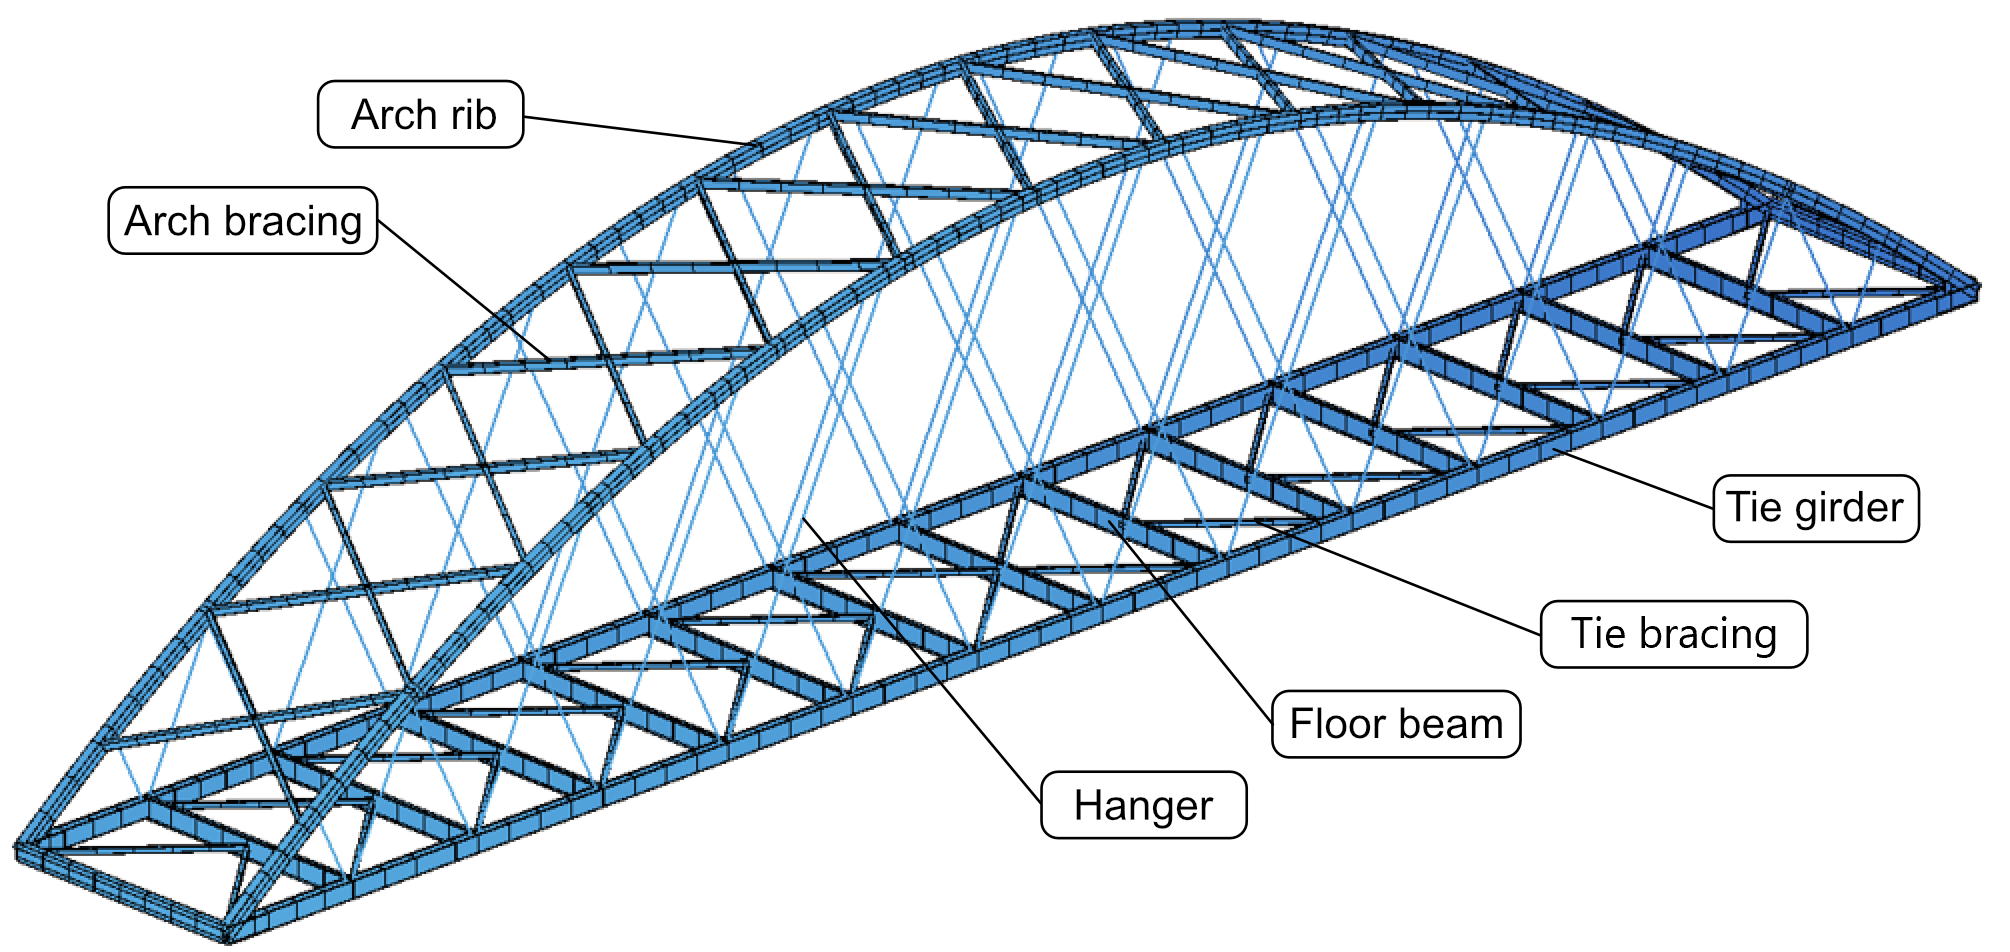
\includegraphics[width=0.65\textwidth]{overleaf/Pictures/illustration_components.PNG}
    \caption{Structural components of a network tied-arch bridge}
    \label{fig:components_illustration}
\end{figure}

The network tied-arch bridge is considered an enhanced construction scheme offering aesthetic appeal and benefits in terms of structural efficiency \cite{Hu}. Steel bridges of this type require significantly less material and allow for more slender cross-sections compared to other more popular bridge types \cite{Herzog}. However, network tied-arch bridges can be considered a complex structural system and the associated challenges are broad and demanding. 
The design of the hanger arrangement and its initial configuration influence the behaviour under asymmetric live loading, fatigue and cable loss. 
Many of these challenges have not been addressed satisfactorily \cite{Bruno}. Further design variables such as the arch shape and its rise as well as its bracing and inclination have barely been studied. Nevertheless, a strong surge in popularity of this bridge type is observed in the last two decades as shown in Fig. \ref{fig:yearly_bridges}.

\begin{figure}[H]
    \centering
    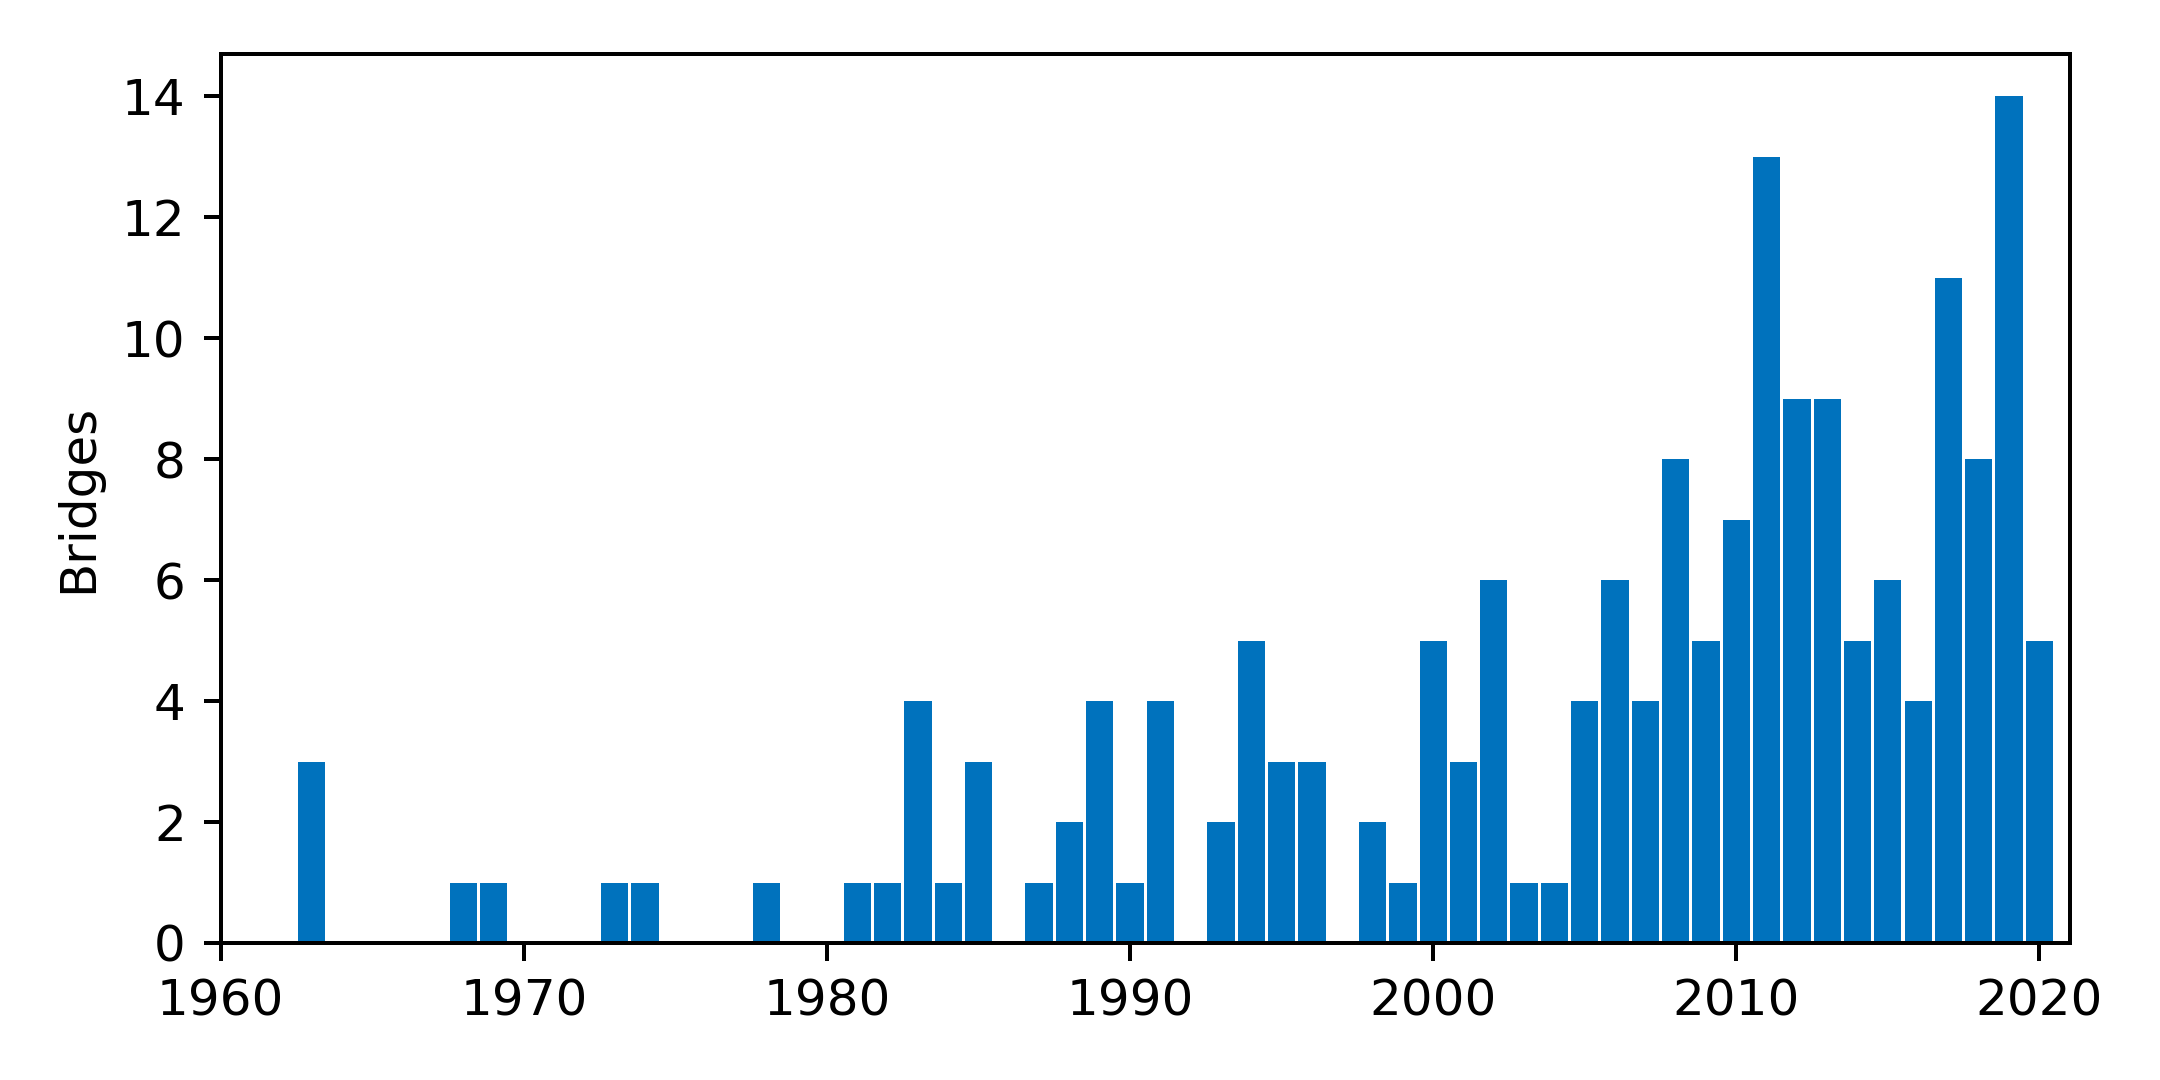
\includegraphics[trim={0 2.2cm 0 1.8cm},clip, width=0.61\textwidth]{overleaf/Pictures/myplot.png}
    \caption{Number of network tied-arch bridges built per year \cite{Cavegn}}
    \label{fig:yearly_bridges}
\end{figure}

The origin of this bridge type can be traced back into the 19th century, when multiple engineers started designing tied-arch bridges featuring a tension chord in the tie. Among these engineers are Joseph Langer and Hermann Lohse who arranged the hangers vertically as shown in Fig. \ref{fig:langerscherbalken}. In the 1920s, the Danish engineer Octavius F. Nielsen recognised the advantages of inclined hangers, which significantly reduce the longitudinal bending moments and thereby allow for longer spans. Despite showing intersecting hangers in his patent document, he only designed hanger arrangements without intersections \cite{Tveit}. The structural analysis of a bridge with intersecting hangers was too challenging at the time. Besides that he struggled with hanger loss due to unloading. One of his bridges is presented in Fig. \ref{fig:nielsenbridge}. \\

\begin{figure}[H]
\centering
\begin{minipage}{.5\textwidth}
  \centering
  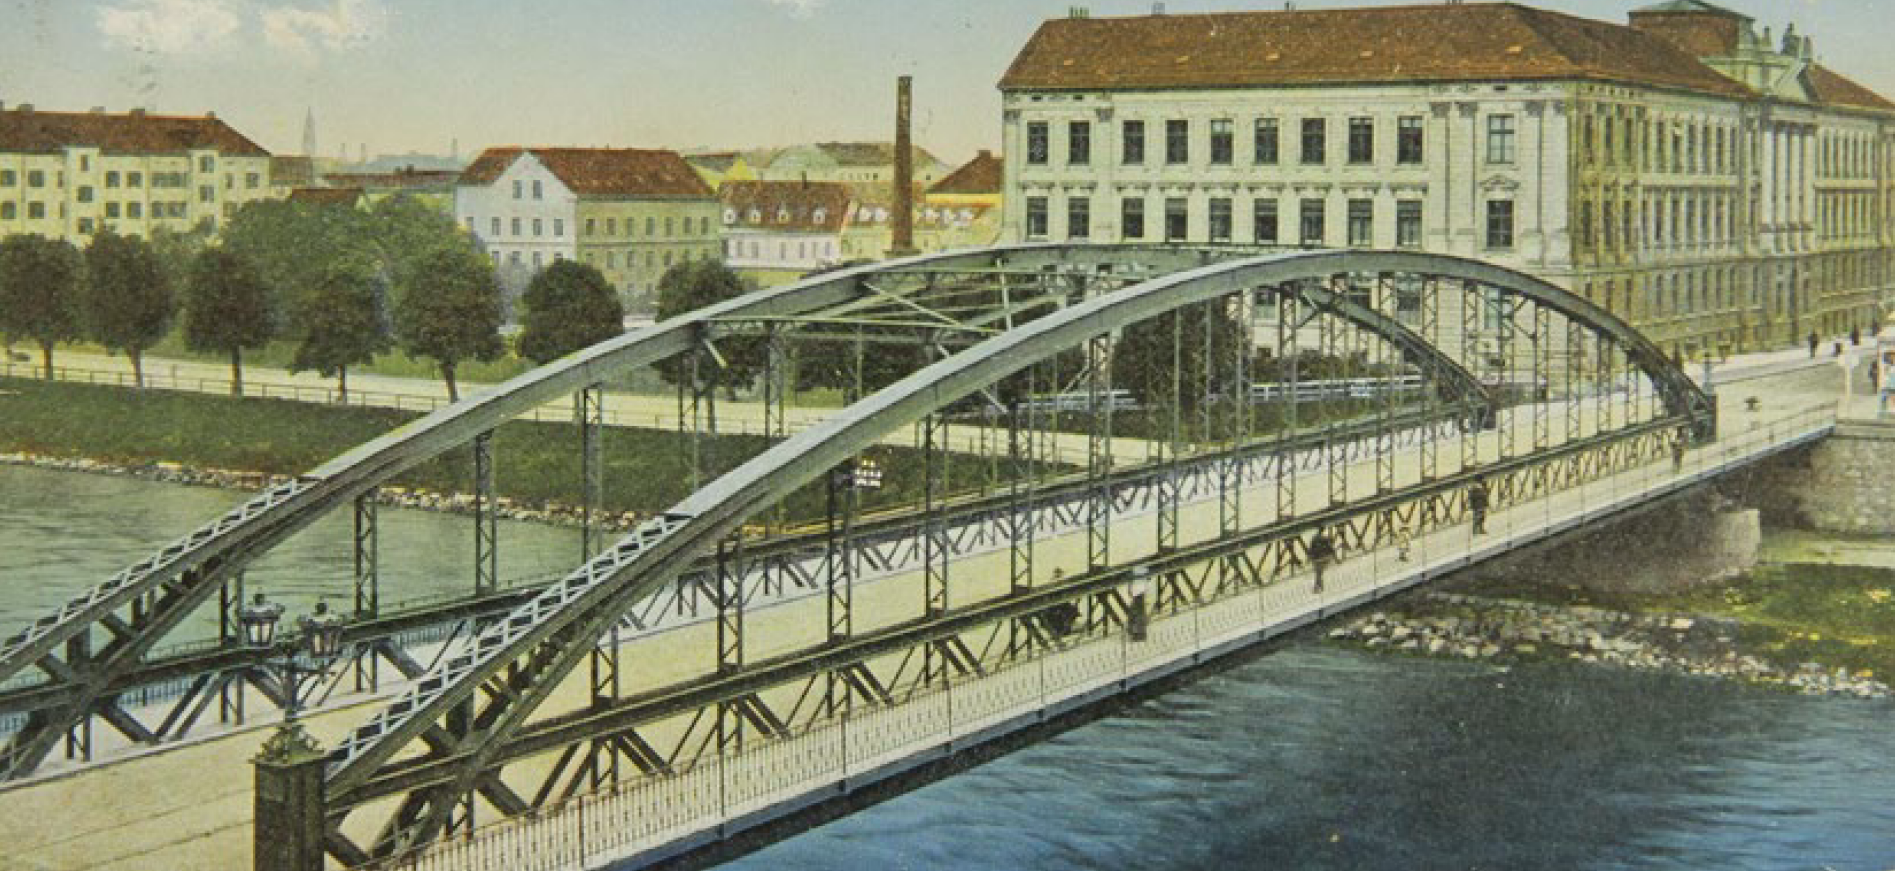
\includegraphics[width=.9\textwidth]{overleaf/Pictures/langerscher balken.PNG}
  \captionof{figure}{Old Ferdinandbridge \cite{Langer}}
  \label{fig:langerscherbalken}
\end{minipage}%
\begin{minipage}{.5\textwidth}
  \centering
  \vspace*{0.6cm}
  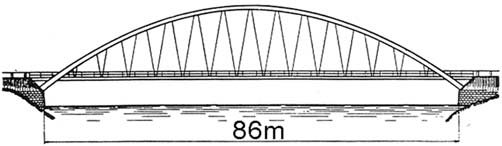
\includegraphics[width=.9\textwidth]{overleaf/Pictures/Nielsen bridge.png}
  \vspace*{0.6cm}
  \captionof{figure}{Nielsen bridge \cite{Nielsen}}
  \label{fig:nielsenbridge}
\end{minipage}
\end{figure}

As the live loading increased in the following years the Nielsen-bridges became less suitable. Only by intersecting the hangers, flat hanger inclinations could be obtained, which solve the problem of hanger unloading. The network tied-arch bridge featuring hangers with multiple intersections was introduced by Per Tveit in 1955. The first bridges of this type were built in 1963. One of them, the Fehmarn Sound Bridge, which already spanned \SI{248}{m}, is shown in Fig. \ref{fig:Fehmarnsundbrücke}.

\begin{figure}[H]
    \centering
    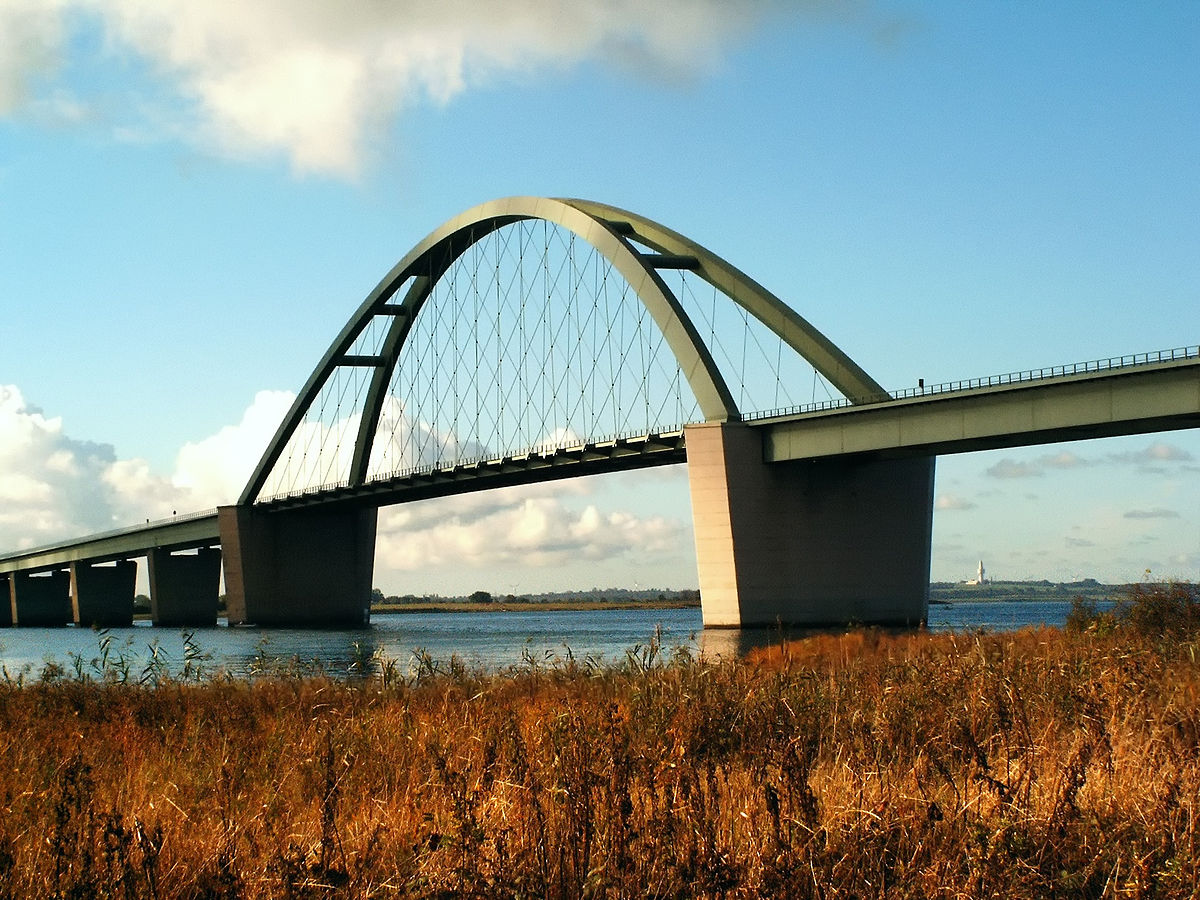
\includegraphics[width=0.6\textwidth]{overleaf/Pictures/Fehmarnsund.jpg}
    \caption{Fehmarn Sound Bridge \cite{Fehmarnsund}}
    \label{fig:Fehmarnsundbrücke}
\end{figure}

In the following decades, Per Tveit focused his research on this bridge type, with particular emphasis on the hanger inclination. Despite his efforts, no more bridges of this type were built in Europe until the end of the millennium. However, the idea was exported to Japan, where it became a relevant alternative to classic tied-arch bridges and over 50 bridges of this type were built. In the last two decades, researchers as well as engineers developed more interest in this bridge type, which has now been built more than 200 times around the world. The Blennerhassett Island Bridge (2006), shown in Fig. \ref{fig:Blennerhassett}, is a particularly large example, which serves as a reference for the investigations in this Thesis.

\begin{figure}[H]
    \centering
    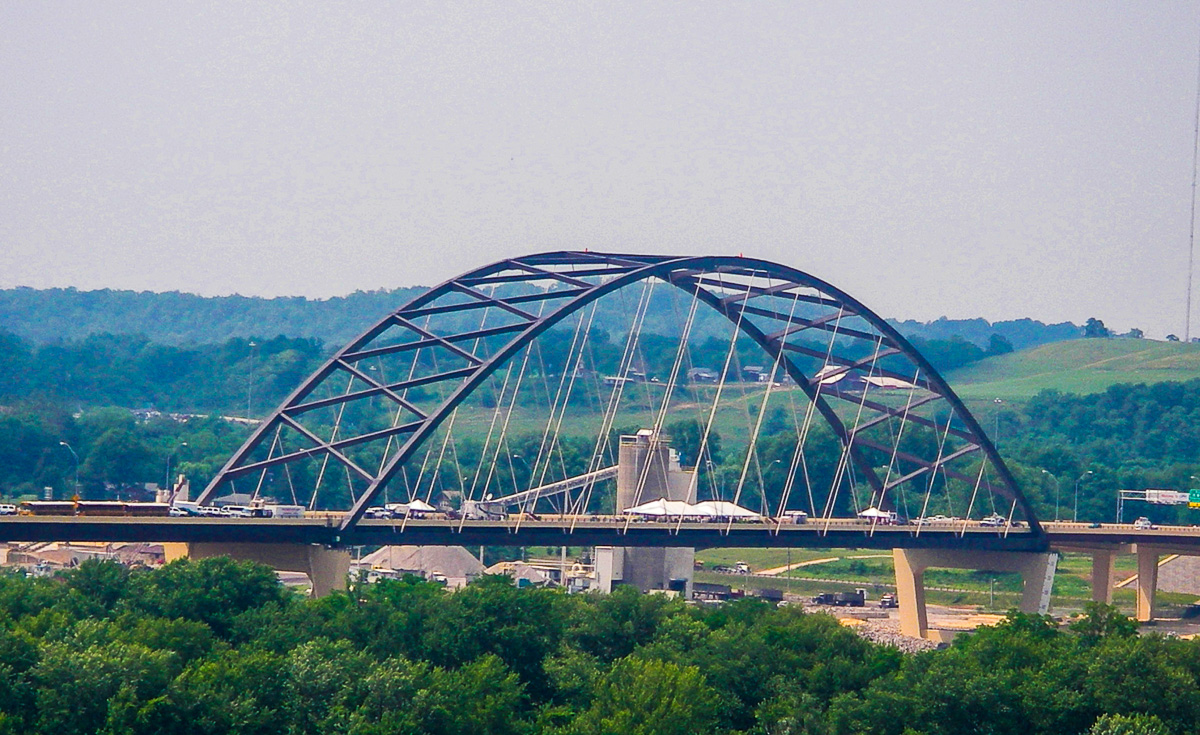
\includegraphics[width=0.6\textwidth]{overleaf/Pictures/Blennerhassett.jpg}
    \caption{Blennerhassett Island Bridge \cite{Blennerhassett}}
    \label{fig:Blennerhassett}
\end{figure}

\subsection{Problem statement} \label{sec:int_prob}
This Master Thesis is part of a series of projects on network tied-arch bridges carried out at the institute of structural engineering at ETH Zurich. As the full optimisation of this bridge type covers too many aspects for a single Thesis, different focal points are investigated independently. A previous Master Thesis carried out by Riccardo Cavegn investigated the arch geometry, the optimal determination of the initial configuration (self-equilibrium stress state) and the hanger inclination. The present Thesis relies on this previous work and faces many identical challenges. Again, the hangers are subject to the optimisation in this Thesis as they determine the fundamental behaviour of this bridge type. In particular, the emphasis lies on the investigation of the hanger density and its related aspects. The Blennerhassett Island Bridge serves as a reference for the investigations. It is an impressive structure which was designed mainly for structural efficiency, which frames the objective in this Thesis.  
%Along with the hanger arrangement, the hanger density is the key parameter determining the fundamental behaviour of this bridge type.\\

\subsection{Outline} \label{sec:int_out}


\subsection{Terminology} \label{sec:int_term}
[Hanger inclination]
[Hanger set]
[Hanger arrangements]
[Knuckle]
[dead to live load ratio]
[zero-displacement method]
[Hanger orientation, left, right]
objective
design condition
self equilibrium stress state
arch shape
          

\newpage
\section{Literature review}\label{sec:review}
In this chapter, previous work on the optimization of network tied-arch bridges is summarized. In Section \ref{sec:rev_arr} it is shown how the different hanger arrangements evolved and which objectives are considered aiming to determine an optimal arrangement. Fundamentally, two approaches are taken for this investigation. On the one hand, parametric studies allow determining the critical parameters. On the other hand, optimization methods have been used not just to identify the tendencies, but to optimize the choice of parameters in the continuous domain. Few authors have taken a further step and introduced a design methodology allowing for a fast and approximately optimized design, which are presented in Section \ref{sec:rev_meth}. While it has received much attention for cable-stayed bridges, cable loss in network tied-arch bridges is only considered scarcely and isolated from the previously mentioned work.[As cen be deciding for design] The corresponding literature is summarized in Section \ref{sec:rev_cable}. Ultimately, the Master Thesis of Riccardo Cavegn, which builds the foundation of this Thesis, is summarized in Section \ref{sec:rev_prev} and a summary of this chapter is given in Section \ref{sec:rev_sum}.

\subsection{Hanger arrangements}\label{sec:rev_arr}
\paragraph*{Hanger unloading}
Per Tveit, described the concept of network tied-arch bridges in his dissertation in 1959. He designed two of the first bridges of this type in 1963 in Norway. In these early stages, only the parallel hanger net and the constant change of inclination pattern are used. Since then, he has been giving lectures around the world to contribute to the broader use of network tied-arch bridges. He points out the various advantages over vertical hangers in terms of lower steel weights, simple detailing and the good use of strong materials \citep{Tveit}. He recommends constant hanger spacing on the arch with one hanger per node to minimize the bending moments in the arch. In \cite{Tveit3} he also conducted investigations on the hanger arrangement, aiming to prevent hanger unloading which is a critical issue under asymmetric loading for short-span bridges. It is found that whereas flat inclinations are more suitable to prevent hanger unloading, they also result in higher hanger forces. To find a solution for these opposing objectives he developed a diagram, presented in Figure \ref{fig:Tveit2}, which predicts the maximum hanger inclination without hanger unloading depending on the ratio of life to dead loads and the loaded length. As a first optimization of the hanger arrangement, it is proposed to increase the inclinations of the hangers as much as possible before the first hanger unloading occurs.

\begin{figure}[H]
    \centering
    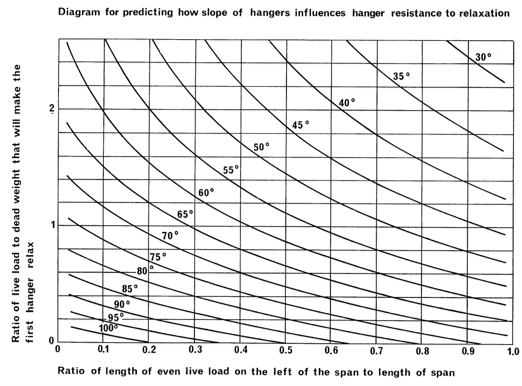
\includegraphics[width=0.6\textwidth]{Pictures/MaximumHangerInclination.png}
    \caption{Indication of the first hanger relaxation (adopted from \citep{Tveit3})}
    \label{fig:Tveit2}
\end{figure}

%Later, he proposed an arrangement with constant distances between the hanger connection points in the middle of the tie, as shown in \autoref{fig:Tveit}. While the nodes on the arch are spaced equidistantly, the connection points on the tie are constructed with the help of an inclined ellipse and an abscissa and an ordinate depending on the parameters $p_1$ and $p_2$. To determine the points on the tie, linearly spaced vertical lines are drawn to the ellipse. The locations of the nodes on the tie are then determined from the ordinate values of the intersection points.\\
%\begin{figure}[H]
%\centering
%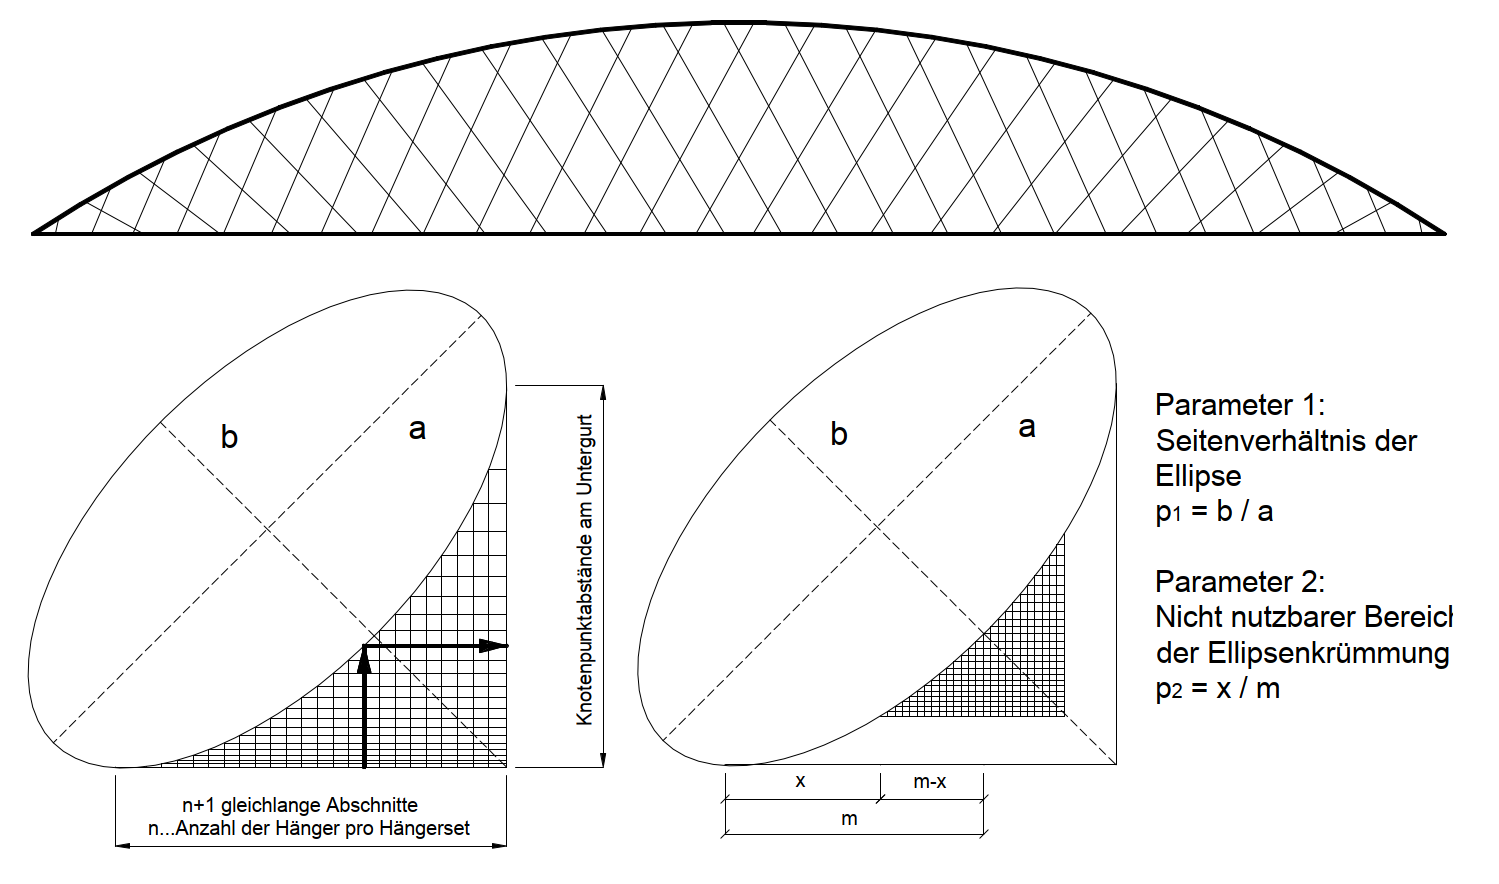
\includegraphics[width=0.7\textwidth]{Pictures/ArrangementTveit.PNG}
%\caption{Arrangement with constant distances in the middle of the tie (adopted from \cite{Teich}).}
%\label{fig:Tveit}
%\end{figure}

\paragraph*{I don't know}
In the new millennium, Tveit supervised multiple Master Theses aiming to optimize the design of network-tied arch bridges. In \citep{BrunnSchanack} [nochmals lesen was da genau gemacht wurde]. They developed the radial arrangement aiming to have a pattern which optimally complies with a circular arch. In the radial arrangement, the hangers are equally spaced on the arch and two following hangers cross each other symmetrically to the radius as shown in \autoref{fig:Brunn}. It was the intention, that if the hanger forces are uniform, the thrust line also approximately corresponds to a circle, resulting in an efficient use of the arch. In the literature, this arrangement is either described by the angle $\alpha$ between the arch and the hanger or by the angle $\beta$ between the hangers and the radius at the first intersection point.

\begin{figure}[H]
\centering
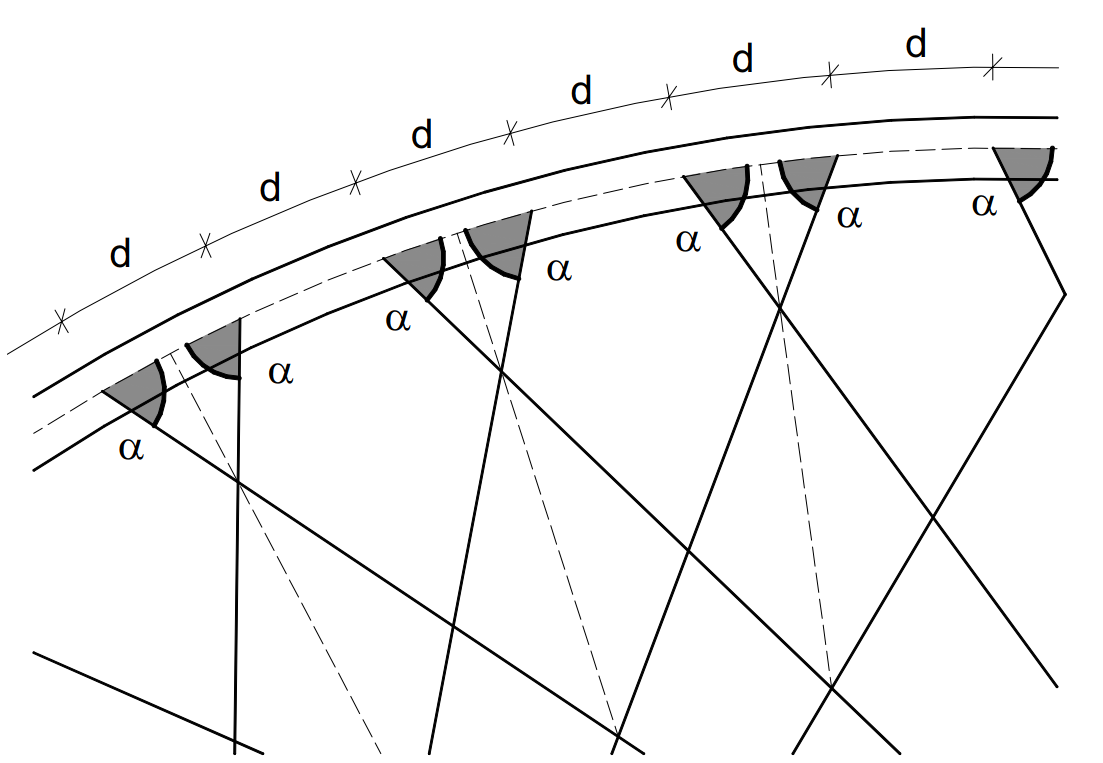
\includegraphics[width=0.4\textwidth]{Pictures/RadialArrangement.PNG}
\caption{Radial hanger arrangement (adopted from \citep{BrunnSchanack2}).}
\label{fig:Brunn}
\end{figure}

Both of the authors continued their work in the field of network tied-arch bridges and conclude their findings in \citep{BrunnSchanack2}. Besides the bending moments and the maximum hanger forces, also the variation of hanger forces, which are relevant for fatigue, and the elastic embedding of the arch is focused on. These objectives are evaluated manually/arbitrarily. In a comparison of the different hanger patterns, it is concluded that parallel hangers are disadvantageous concerning the bending moments in the arch as the hanger forces vary strongly. Angles of inclination between $55\degree$ and $60\degree$ give the best results. For the constant change of inclination arrangement the middle hanger was recommended to be inclined in the similar range from $56\degree$ to $60\degree$. Further, the change of inclination between two following hangers should lead to an inclination of up to $80\degree$ in the steepest hangers. The radial arrangement was considered optimal, especially for the small corresponding variation of maximum hanger forces and uniform embedding of the arch. The angle between the hangers and the arch are recommended to be between $55\degree$ and $60\degree$. Interestingly, the optimal solutions for each hanger arrangement feature a middle hanger with an inclination of $55\degree$ to $60\degree$. Further, it is recommended that the hanger spacing on the arch lies between \SI{2.5}{m} and \SI{4}{m}.

\paragraph*{Hanger forces}
To judge the objectives mathematically \citep{Teich} conducted a vast parameter study varying the key in-plane parameters. Its focus lies on the objectives related to the hangers which are combined into a scaled dimensionless score. Namely, these objectives are the maximum force and its variation, the cyclic stresses and the amount of unloaded cables. In the evaluation of these objectives the three hangers closest to the arch were disregarded for and it is proposed to design them detached from the general hanger pattern. The parameters such as the span, the rise, the amount of hangers and their arrangement are varied in the study, leading to a total of approximately 90000 variants. The only in-plane parameter that is left constant is the arch shape which is always modelled circular. Based on the normalized and combined results, a design methodology was developed which is explained in Section \ref{sec:rev_meth}. For the parallel hanger pattern smaller angles of inclination between $50\degree$ and $55\degree$ are recommended. However, hanger unloading poses a serious issue for this arrangement. The constant change of inclination arrangement generally relies on large changes of the inclination and yields the best results with respect to the cyclic stresses and hanger unloading. The radial arrangement performed well in all objectives, especially if the amount of hangers is rather low. It gave the best results overall and Teich recommends intersection angles around $36\degree$. For some cases also the arrangement with equidistant spacing on the tie proofed efficient. In this pattern, optimal results were obtained by a variety of values for the two parameters.
%results normalized and mixed multiple times.
%no prestressing
\paragraph*{Fatigue}
The assumption that the hangers close to the knuckles should be designed independently from the overall pattern agrees with \citep{Pellegrino}. In this study various hanger patterns are evaluated with respect to fatigue. The considered hanger patterns are the constant change of slope and the radial arrangement which are also compared to an arrangement with vertical hangers. It is found that with respect to the cyclic stresses, vertical hangers are superior over network arrangements. By inclining the vertical hangers the behaviour deteriorates strongly and improves again for flat inclinations. Especially the flat hangers near the knuckle undergo very high cyclic stresses and various arrangements to improve this issue are studied. However, none of the adapted arrangements provided better results independent of the intersecting angle. Steeper hangers near the knuckles are generally a good advice to start with. For a radial hanger arrangement with an intersecting angle of $35\degree$, it is recommended to arrange the last five hangers of each set parallel to the previous one, as shown in \autoref{fig:Pellegrino}. This advice has to be judged considering that a high amount of 22 hangers per set without prestressing were used in the study.

\begin{figure}[H]
    \centering
    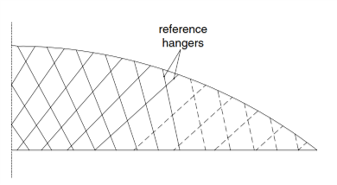
\includegraphics[width=0.5\textwidth]{Pictures/PellegrinoArrangement.png}
    \caption{Modified radial arrangement (adapted from \citep{Pellegrino})}
    \label{fig:Pellegrino}
\end{figure}

\paragraph*{Numerical optimization}
Recently, many researchers have focused on numerical optimization methods over parametric studies. Technically, all parameters describing the scheme of a network tied arch bridge can be considered. However, as it is usually not the aim to optimize the entire design process, researchers prefer to limit the process to a few key variables. As some of the parameters are of discrete form, the problem is mathematically described as a constrained mixed-integer problem. Genetic algorithms with penalization provide an efficient and often used tool for these problems. In \citep{Belevicius}, an optimal pedestrian bridge scheme with respect to weight minimization is obtained for different spans. Even with the rather limited amount of nine parameters, the optimized sets are well dispersed over the feasible domain, illustrating the multi-modality of the underlying problem.
It also demonstrates well the difficulties associated with numerical optimization for design purposes. Even after reducing the amount of parameters, the results do not resemble typical tied-arch bridges, be it for the high amount of hangers or the large rise-to-span ratio. The aim of finding a simple and fast method for obtaining the full initial design is therefore reached only in an unsatisfactory manner. Ultimately, It a strongly varying hanger pattern is recommended as well as a rise-to-span ratio of 0.2 to 0.23. The hanger spacing on the tie should be shorter for the steep hangers and increase towards the other side.\bigskip

In \citep{Tan} a pedestrian bridge with a sparse hanger arrangement was investigated using an evolutionary optimization procedure. Each hanger is arranged independently of an overall arrangement. It was found that an arrangement approximately consisting of two separate patterns reduced the internal forces in the arch and the tie the most. Near the knuckles vertical hangers and in the span approximately parallel hangers resulted as shown in \autoref{fig:Tan}.

\begin{figure}[H]
\centering
\begin{subfigure}{0.5\textwidth}
    \centering
    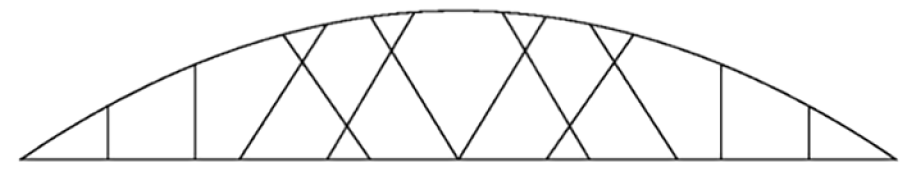
\includegraphics[width=0.9\textwidth]{Pictures/Tan 1.PNG}
\end{subfigure}%
\begin{subfigure}{.5\textwidth}
    \centering
    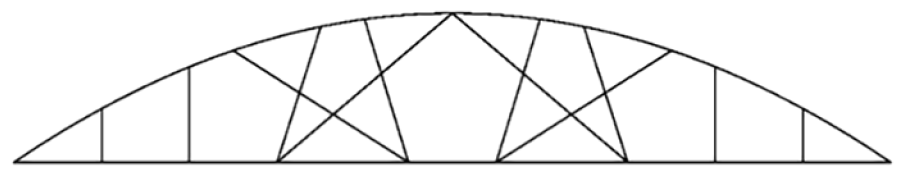
\includegraphics[width=0.9\textwidth]{Pictures/Tan 2.PNG}
\end{subfigure}
\caption{Optimal sparse hanger arrangements (adopted from \cite{Tan}).}
\label{fig:Tan}
\end{figure}

%[Ostrycharczyk] %Adapted radial pattern for equidistant hanger spacing on tie. Highly important that hangers don't lie to close to each other on the arch.


\subsection{Design methodologies} \label{sec:rev_meth}

In a first step the number of hangers is chosen according to the recommended values shown in [Figure]. Using the amount of hangers and the span the optimal hanger arrangement pattern is chosen using a different table. For all cases either the constant change of inclination or the radial arrangement are the preferred choice. In Tables corresponding to the hanger arrangement pattern the best set of parameters can be chosen depending on the amount of hangers. An example for the radial arrangement is shown in [Figure]. The three hangers closest to the knuckle should ultimately be designed manually. They were also excluded in the evaluation of the objectives.
%[Bruno]
%[Teich]

\subsection{Cable loss} \label{sec:rev_cable}
Most of the work dedicated on cable loss focuses on cable-stayed bridges. There, it is not unusual for this accidental limit state to govern the design of the superstructure. In \citep{Wolff} is found that the loss of two or more cables can impair the global stability of a cable-stayed bridge.
[give guidelines for cable-stayed bridges?]
In \citep{Zoli} a parametric sensitivity study on cable loss for the Blennerhassett Island Bridge is conducted. [Kann man diese Publikation irgendwo finden?]
It is concluded that cable loss should be a key consideration for the design process for all major bridges.\bigskip

In \citep{Bruno}, a study on the behaviour of network tied-arch bridges is conducted to identify the key factors on the impacts. The behaviour is studied using the simplified approaches of the PTI and the Eurocode and compared to a dynamic non-linear FE-analysis. As a base case, a bridge with a span of \SI{180}{m} and a rise of \SI{30}{m} is studied featuring a parallel hanger arrangement with 17 hangers per set and an inclination of $65 \degree$. Whereas the prestressing is taken into account using the "zero-displacement method"/the methodology by Bruno.

It was found that the most dangerous cables to lose are the ones located near the quarter points of the tie and inclined towards the middle of the arch. The corresponding vertical displacements are maximal for this hanger with a value of $l/4000$. The stresses in the neighbouring hangers of the same set increase by 60\% if the cable at the quarter point is lost. The hangers of the other set are less affected increasing by a maximum of less than 25\% as shown in Fig. \ref{fig:Bruno}. Further, he found that parallel arrangements with flatter inclinations cause the displacements and the internal forces to increase. Restricted to the plausible range of $50\degree$ to $70\degree$ differences amounting up to 20\% can be expected. In Figure [] the respective displacements are also compared to the arrangement with vertical hangers, where also the resulting total volumes of the hangers are given. It is seen that the vertical arrangement performs much butter despite using a smaller amount quantity of cable material. Overall it is concluded that also the simplified methods provide an adequate degree of accuracy.

\begin{figure}[H]
    \centering
    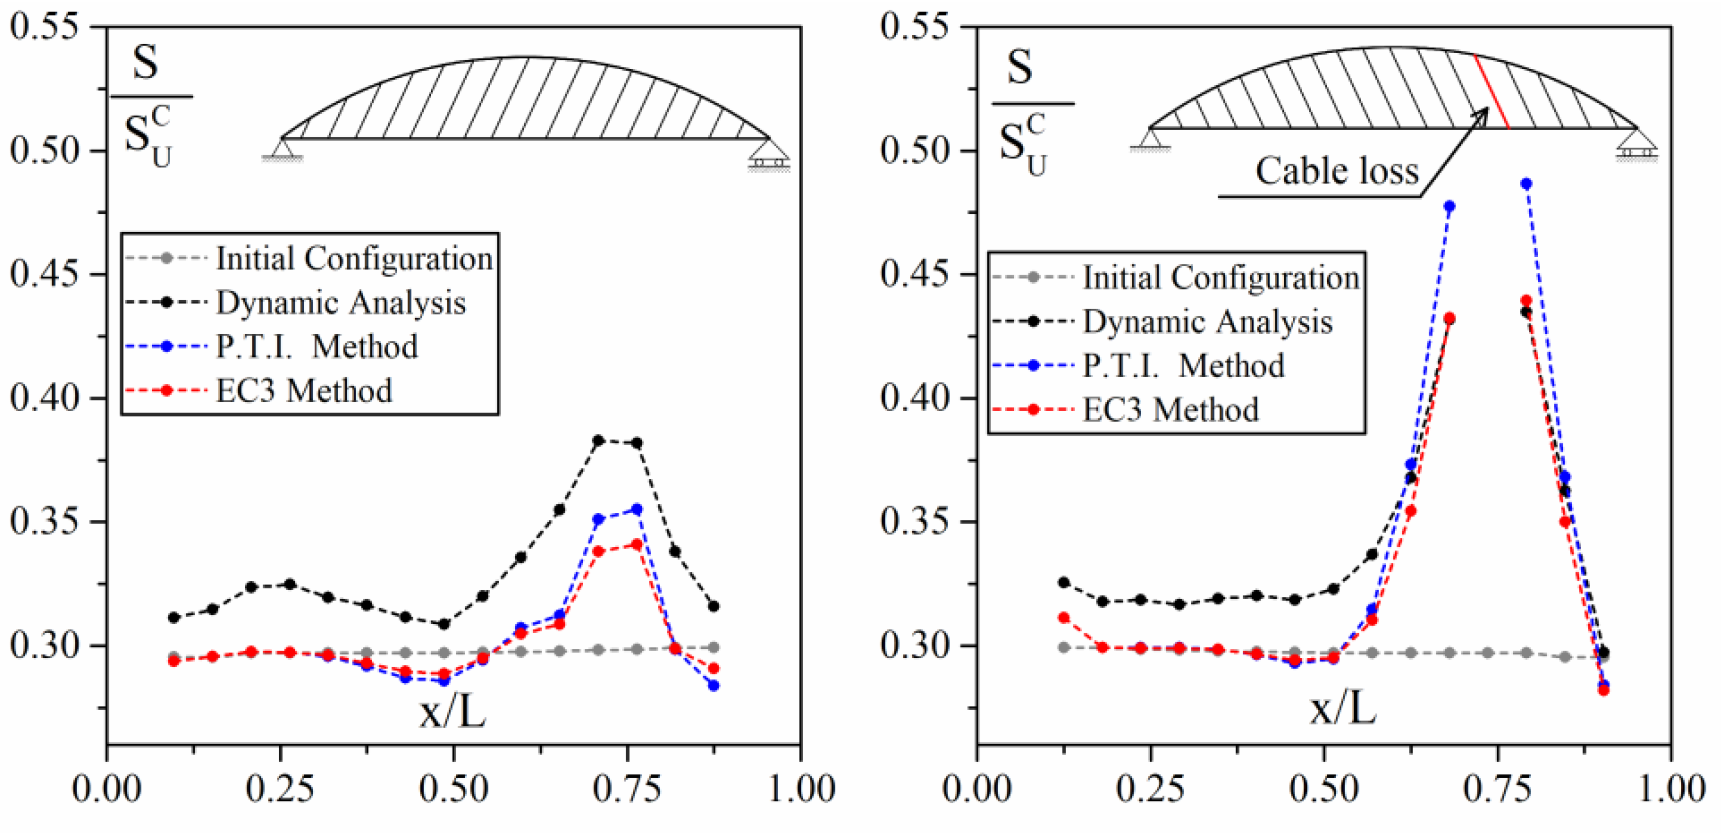
\includegraphics[width=0.75\textwidth]{Pictures/BrunoCableLoss.PNG}
    \caption{Stress distribution in the hanger sets (adopted from \citep{Bruno})}
    \label{fig:Bruno}
\end{figure}

\begin{figure}[H]
    \centering
    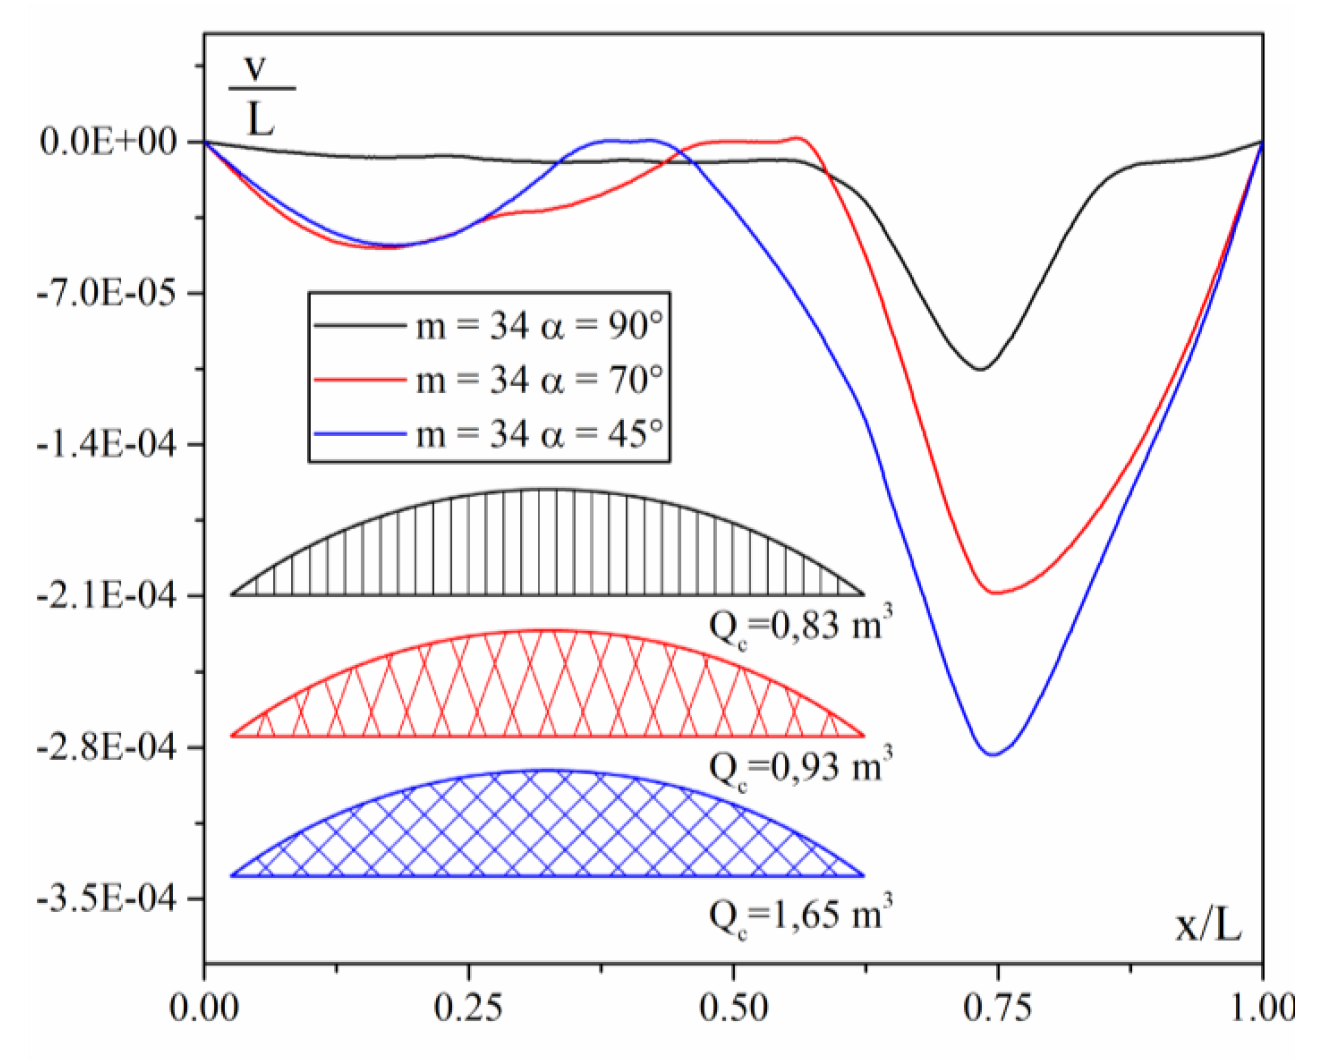
\includegraphics[width=0.6\textwidth]{Pictures/BrunoArrangements.PNG}
    \caption{Comparison between vertical and network cable systems (adopted from \citep{Bruno})}
    \label{fig:Bruno2}
\end{figure}

%[Islam] Considers material costs agrees with optimal inclination

\newpage
\subsection{Previous work in this series}\label{sec:rev_prev}
In a previous Master's Thesis at the Chair of Structural Engineering for Concrete Structures and Bridge Design, Riccardo Cavegn investigated the optimal arch geometry \citep{Cavegn}. Its dependency on the hanger arrangement was studied in particular with the Blennerhassett Island Bridge as a reference bridge. As a hanger pattern, the constant change of inclination arrangement was investigated in a parameter study. Two examples are shown in Fig. \ref{fig:Cavegn1} and Fig. \ref{fig:Cavegn2}, the latter corresponds to the special case of a parallel hanger pattern with parallel hangers.

\begin{figure}[H]
\centering
\begin{subfigure}{0.5\textwidth}
    \centering
    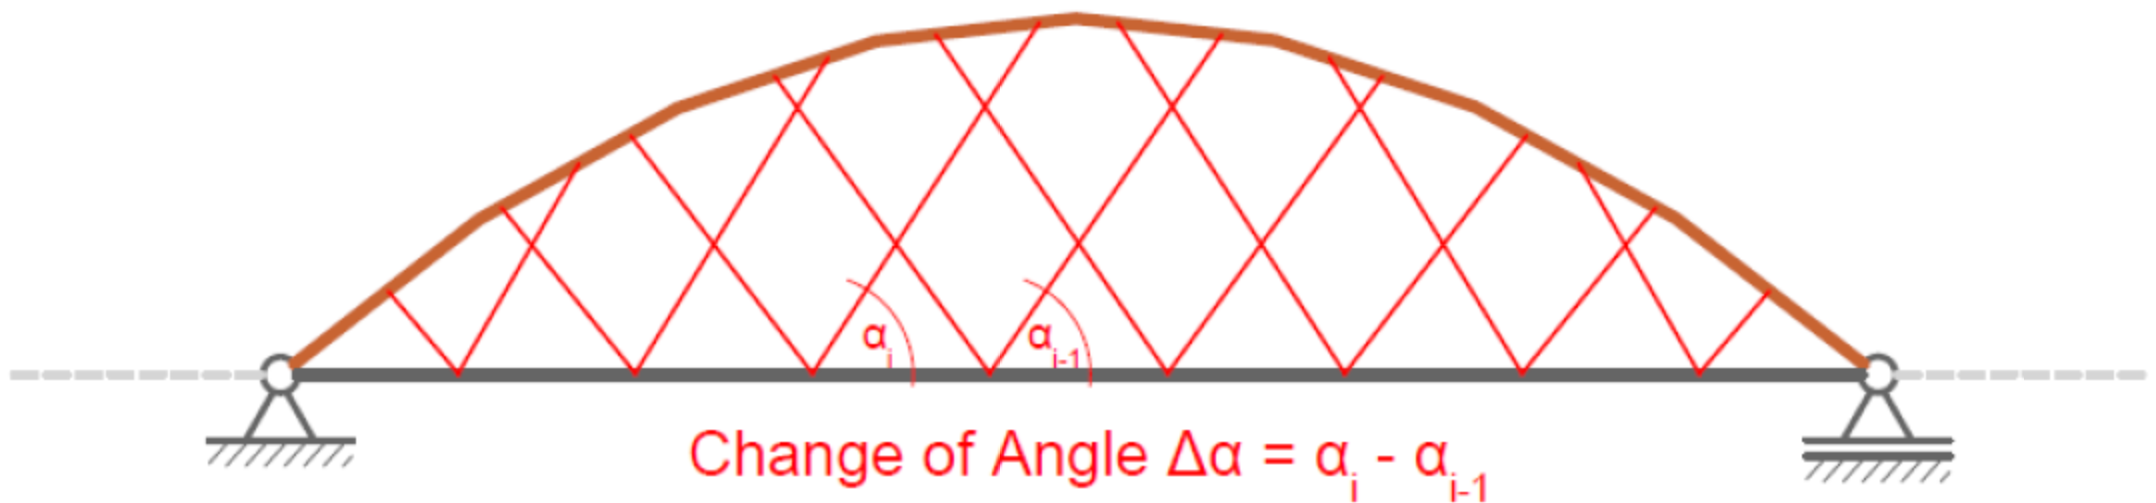
\includegraphics[width=0.9\textwidth]{Pictures/ConstantChangeCavegn.PNG}
    \caption{Constant change of inclination arrangement}
    \label{fig:Cavegn1}
\end{subfigure}%
\begin{subfigure}{.5\textwidth}
    \centering
    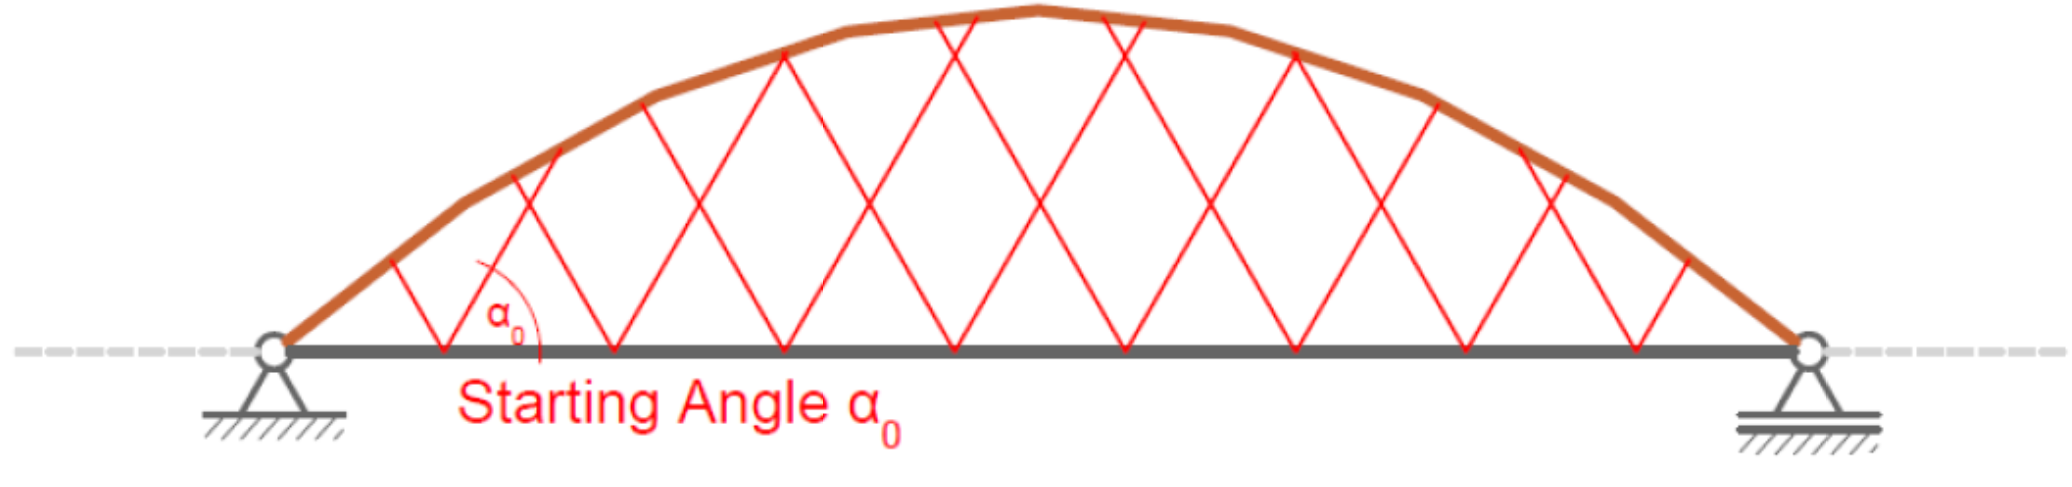
\includegraphics[width=0.9\textwidth]{Pictures/ParallelArrangementCavegn.PNG}
    \caption{Parallel arrangement}
    \label{fig:Cavegn2}
\end{subfigure}
\caption{Hanger arrangements and their parameters (adopted from \cite{Cavegn}).}
\label{fig:Cavegn}
\end{figure}

In the first step, the prestressing of the hangers was determined to minimize the bending moments under dead loads. To achieve this the hanger tuning matrix relating the individual unit strains of the hangers to their impacts was calculated using structural analysis software. This matrix was then used to calculate the prestrains giving minimal bending moments in the tie girder as shown in \autoref{fig:Cavegn3}. In a second step, the obtained normal forces were used to graphically construct the thrust line of the arch as illustrated in \autoref{fig:Cavegn4}. As the two steps influence each other, they are repeated until the obtained arch geometry does not change significantly. It was seen that the obtained arch geometries generally do not correspond to the circular or the parabolic shape. Sometimes they even lie outside of the two traditionally used shapes. By approximating the obtained shape with a quartic function an expression sufficiently close to the thrust line was found. Further, it was seen that flat angles of inclination lead to thrust lines that are more inclined near the bearing. Ultimately, the impacts under 3 live load combinations were used to estimate the costs of the generated structure which was taken as a further objective of the optimization. A flatter hanger inclination turned out to reduce the bending moment in the tie and the arch, whereas the opposite effect was observed in the maximum hanger forces. The estimated costs of the bridge were reduced the most by rapidly decreasing inclinations and high initial inclinations. The cost function was thereby minimized by up to 12\%. However also other patterns, e.g. with constant inclination, were shown to perform well if the arch geometry is adapted to the thrust line.
\begin{figure}[H]
\centering
\begin{subfigure}{0.5\textwidth}
    \centering
    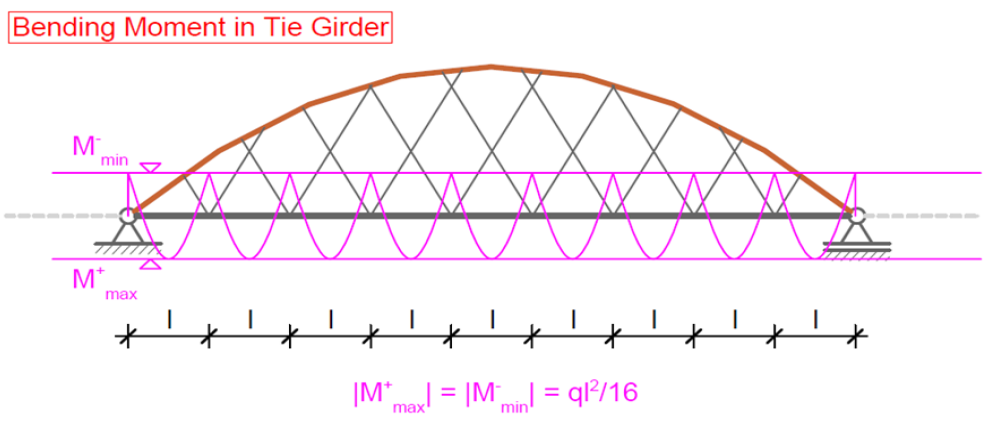
\includegraphics[width=0.73\textwidth]{Pictures/OptimizedBendingMoment.PNG}
    \caption{Determination of the self-equilibrium stress state}
    \label{fig:Cavegn3}
\end{subfigure}%
\begin{subfigure}{.5\textwidth}
    \centering
    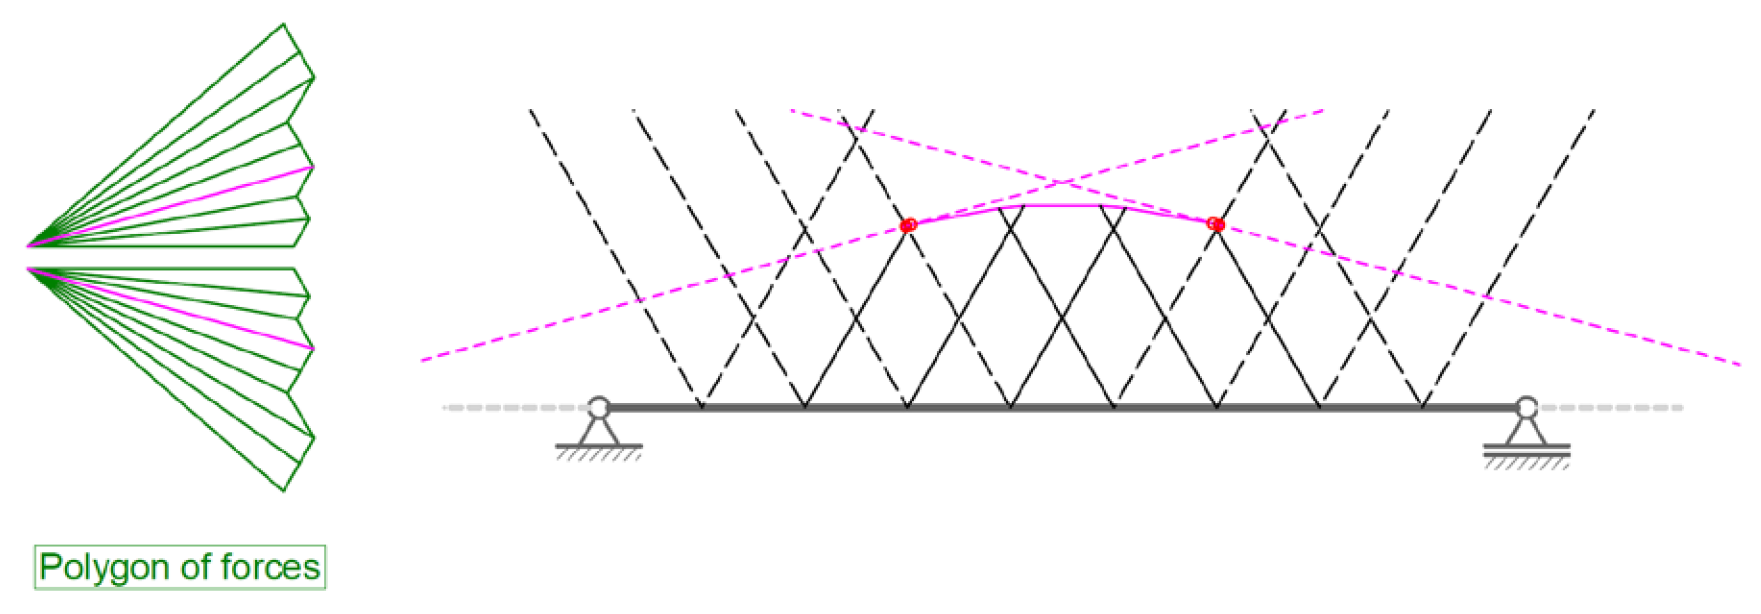
\includegraphics[width=0.9\textwidth]{Pictures/GraphicalThrustLineConstruction.PNG}
    \caption{Graphical construction of the arch shape}
    \label{fig:Cavegn4}
\end{subfigure}
\caption{Optimization steps (adopted from \cite{Cavegn}).}
\label{fig:Cavegn34}
\end{figure}

\newpage
\subsection{Summary} \label{sec:rev_sum}

Further it was pointed out early by \citep{Geissler} that only with a detailed structural model, including accurately modelled knuckles, reliable estimations of the hanger forces can be made.

In the last decade, many researchers have focused on the numerical optimization methods for given conditions. These methods produced efficient solutions for the structurally challenging problems. However, they do not provide practical help to the inexperienced engineer during the (preliminary) design. 
                  

\newpage
\section{Methods}\label{sec:methods}
\subsection{Reference bridges}
%Plane model is appropriate Smit: Design and construction of a railway arch bridge with a network arrangement

\subsection{Structural modelling}

\subsection{Load cases}

\subsection{Self-equilibrium stress state}
% Permanent state

\subsection{Design verification}

\subsection{Estimation of cost function}

\begin{table}[H]
\caption{Ultimate limit state load combinations}
\centering
\begin{tabular}{lccccc}
\hline
Load         & EL  & DC         & DW         & LL   & WS  \\ \hline
Strength-I   & 1.0 & 1.25 / 0.9 & 1.5 / 0.65 & 1.75 & -   \\
Strength-III & 1.0 & 1.25 / 0.9 & 1.5 / 0.65 & -    & 1.4 \\ 
Strength-IV  & 1.0 & 1.5        & 1.5        & -    & 1.4 \\ \hline
\end{tabular}
\end{table}



\begin{table}[H] 
\caption{The effects of wind loading per region}
\centering
\begin{tabular}{lccc}
\hline
Region & Normal force & Moment-y & Moment-z \\
 & [kN]   & [kNm] & [kNm] \\ \hline
Arch 1 & -8175 & 668 & 13851\\
Arch 2 & -7793 & -670 & 10749\\
Arch 3 & -4066 & -533 & 2591\\
Arch 4 & -3852 & 117 & 111\\
Tie 1 & 5369 & -2327 & 9653\\
Tie 2 & 7002 & -1109 & 5880\\
Tie 3 & 6152 & 404 & 434\\
Tie 4 & 5275 & 702 & 788\\ \hline
\end{tabular}
\end{table}

\begin{table}[H] 
\caption{The cross-sectional resistances per region}
\centering
\begin{tabular}{lccc}
\hline
Region & Normal force & Moment-y & Moment-z \\
 & [kN]   & [kNm] & [kNm] \\ \hline
Arch 1 & \SI{130000}{} & \SI{78708}{} & \SI{79115}{}\\
Arch 2 & \SI{108768}{} & \SI{71458}{} & \SI{63445}{}\\
Arch 3-4 & \SI{82309}{} & \SI{50017}{} & \SI{42729}{}\\
Tie 1 & \SI{153228}{} & \SI{100810}{} & \SI{76190}{}\\
Tie 2 & \SI{117134}{} & \SI{82766}{} & \SI{56610}{}\\
Tie 3-4 & \SI{100574}{} & \SI{76175}{} & \SI{45792}{}\\ \hline
\end{tabular}
\end{table}

\begin{table}[H] 
\caption{The design verifications}
\centering
\begin{tabular}{cccccl}
\hline
Segment & \multicolumn{4}{c}{Demand / Capacity} & \\
 & Strength-I & Strength-III & Strength-IV & Base case & \\ \hline
Arch 1 & 0.86 & \textbf{1.01} & 0.72 & \textbf{1.01} & () \\
Arch 2 & \textbf{1.18} & 1.13 & 1.00 & \textbf{1.18} & () \\
Arch 3 & \textbf{0.89} & 0.82 & 0.74 & \textbf{0.89} & () \\
Tie 1 & 0.44 & \textbf{0.55} & 0.32 & \textbf{0.55} & () \\
Tie 2 & \textbf{0.51} & 0.47 & 0.37 & \textbf{0.51} & () \\
Tie 3 & \textbf{0.50} & 0.47 & 0.37 & \textbf{0.50} & () \\
Hanger & \textbf{0.98} & 0.83 & 0.63 & \textbf{0.98} & () \\
\hline
\end{tabular}

\end{table}


\begin{table}[H] 
\caption{The design verifications (from design drawings)}
\centering
\begin{tabular}{llcccc}
\hline
Region                  & Limit state  & Normal force & Moment-y & Moment-z & Demand/Capacity \\
                        &              &              &          &          &                 \\ \hline
\multirow{2}{*}{Arch 1} & Strength-III & -70913       & 6360     & 30119    & 0.96            \\
                        & Cable loss   & -56981       & 39583    & 4457     & 1.00            \\ \hline
\multirow{2}{*}{Arch 2} & Strength-III & -70789       & 3831     & 22546    & 1.00            \\
                        & Cable loss   & 56879        & -22025   & -462     & 0.85            \\ \hline
\multirow{2}{*}{Arch 3} & Strength-IV  & -68502       & 8085     & -891     & 0.99            \\
                        & Cable loss   & -53138       & 22706    & 396      & 1.00            \\ \hline
\multirow{2}{*}{Arch 4} & Strength-IV  & -60189       & 5190     & 203      & 0.83            \\
                        & Cable loss   & -48410       & -23510   & 229      & 0.97            \\ \hline
\multirow{2}{*}{Tie 1}  & Strength-III & 55358        & -8760    & -17944   & 0.65            \\
                        & Cable loss   & 50354        & -6058    & -4208    & 0.60            \\ \hline
\multirow{2}{*}{Tie 2}  & Strength-III & 57057        & -3451    & -10469   & 0.69            \\
                        & Cable loss   & 50580        & 2026     & -2225    & 0.61            \\ \hline
\multirow{2}{*}{Tie 3}  & Strength-I   & 51443        & 13565    & -355     & 0.68            \\
                        & Cable loss   & 47511        & 10585    & -315     & 0.88            \\ \hline
\multirow{2}{*}{Tie 4}  & Strength-I   & 54268        & 6565     & 857      & 0.63            \\
                        & Cable loss   & 49624        & 5022     & 384      & 0.76            \\ \hline 
\end{tabular}
\end{table}                   

\newpage
\section{Results}\label{sec:results}

\subsection{Base case}
As a reference for all following calculations, a model representing the Blennerhassett Island Bridge's final design is investigated. The results obtained by the analysis are then compared to the ones in the design drawings for plausibility. A particular challenge is the determination of the self-equilibrium stress state. As the arch was defined as an unsuitable parabola, appropriate hanger forces were determined by trial and error in the design. These permanent hanger forces of the final design are available in the drawings. However, they are unsuitable for calculating the base case, as the load distribution in the model is simplified. Instead of another trial and error procedure for the base case, the hanger forces are obtained as the result of a simultaneous arch and tie moment optimisation. Thereby, the arch's moment is weighed by a factor of 1.5 to achieve an optimal similarity. Further, the hanger forces are bounded between 25\% and 45\% of their nominal strength. The base case's internal force distributions for the permanent state are shown in Fig. \ref{fig:base_case_permanent}. Instead of the normal force in the hangers, the demand over capacity ratio is shown directly. Only the hangers of one set are shown, namely the ones inclined to the right side, and the dots are connected for readability. As a comparison, the extreme values found on the design drawings are also shown.

\begin{figure}[H]
    \centering
    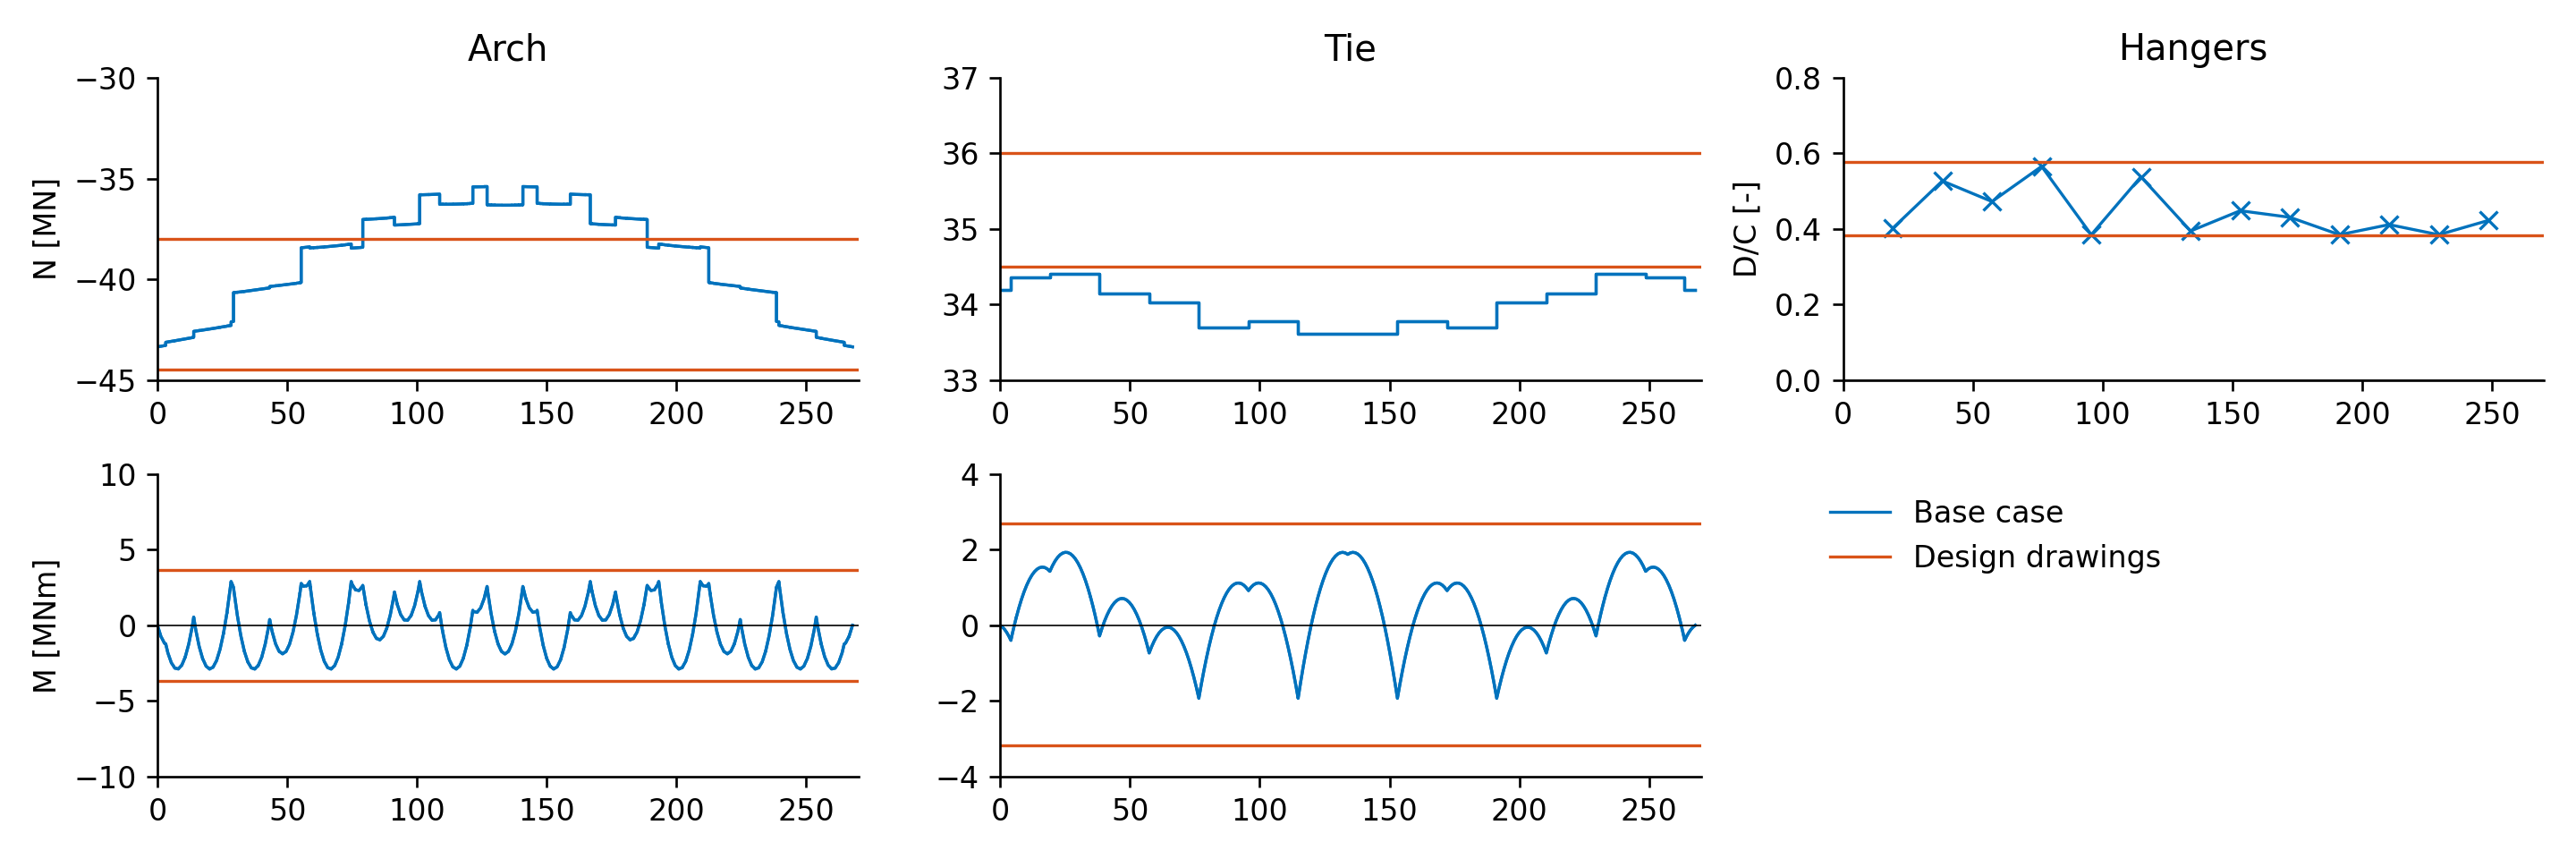
\includegraphics[width=\textwidth]{calculations/Base case/Permanent state.png}
    \caption{Permanent internal forces of the base case and reference values from the drawings}
    \label{fig:base_case_permanent}
\end{figure}

It can be seen that the moment distributions in the arch and the tie, as well as the normal forces in the hangers, match the design drawings very well. Only for the normal force in the arch rib and the tie girder an offset of \SI{2}{MN} can be observed. This difference is probably due to underestimating the weight of the bridge and its simplified assignment to the beams. However, overall the obtained internal force distribution matches the design drawings sufficiently well. It can be concluded, that for a fixed arch shape the simultaneous arch and tie moment optimisation yields adequate results.\medskip

Another comparison is drawn between the effects under characteristic live loads. As there are countless live load combinations, which are to be accounted for, it makes sense to look at the entire ranges of possible internal forces. They are shown in Fig. \ref{fig:base_case_live} by the two blue lines representing the lower and the upper limit. They are compared to the extreme values found in the design drawings.

\begin{figure}[H]
    \centering
    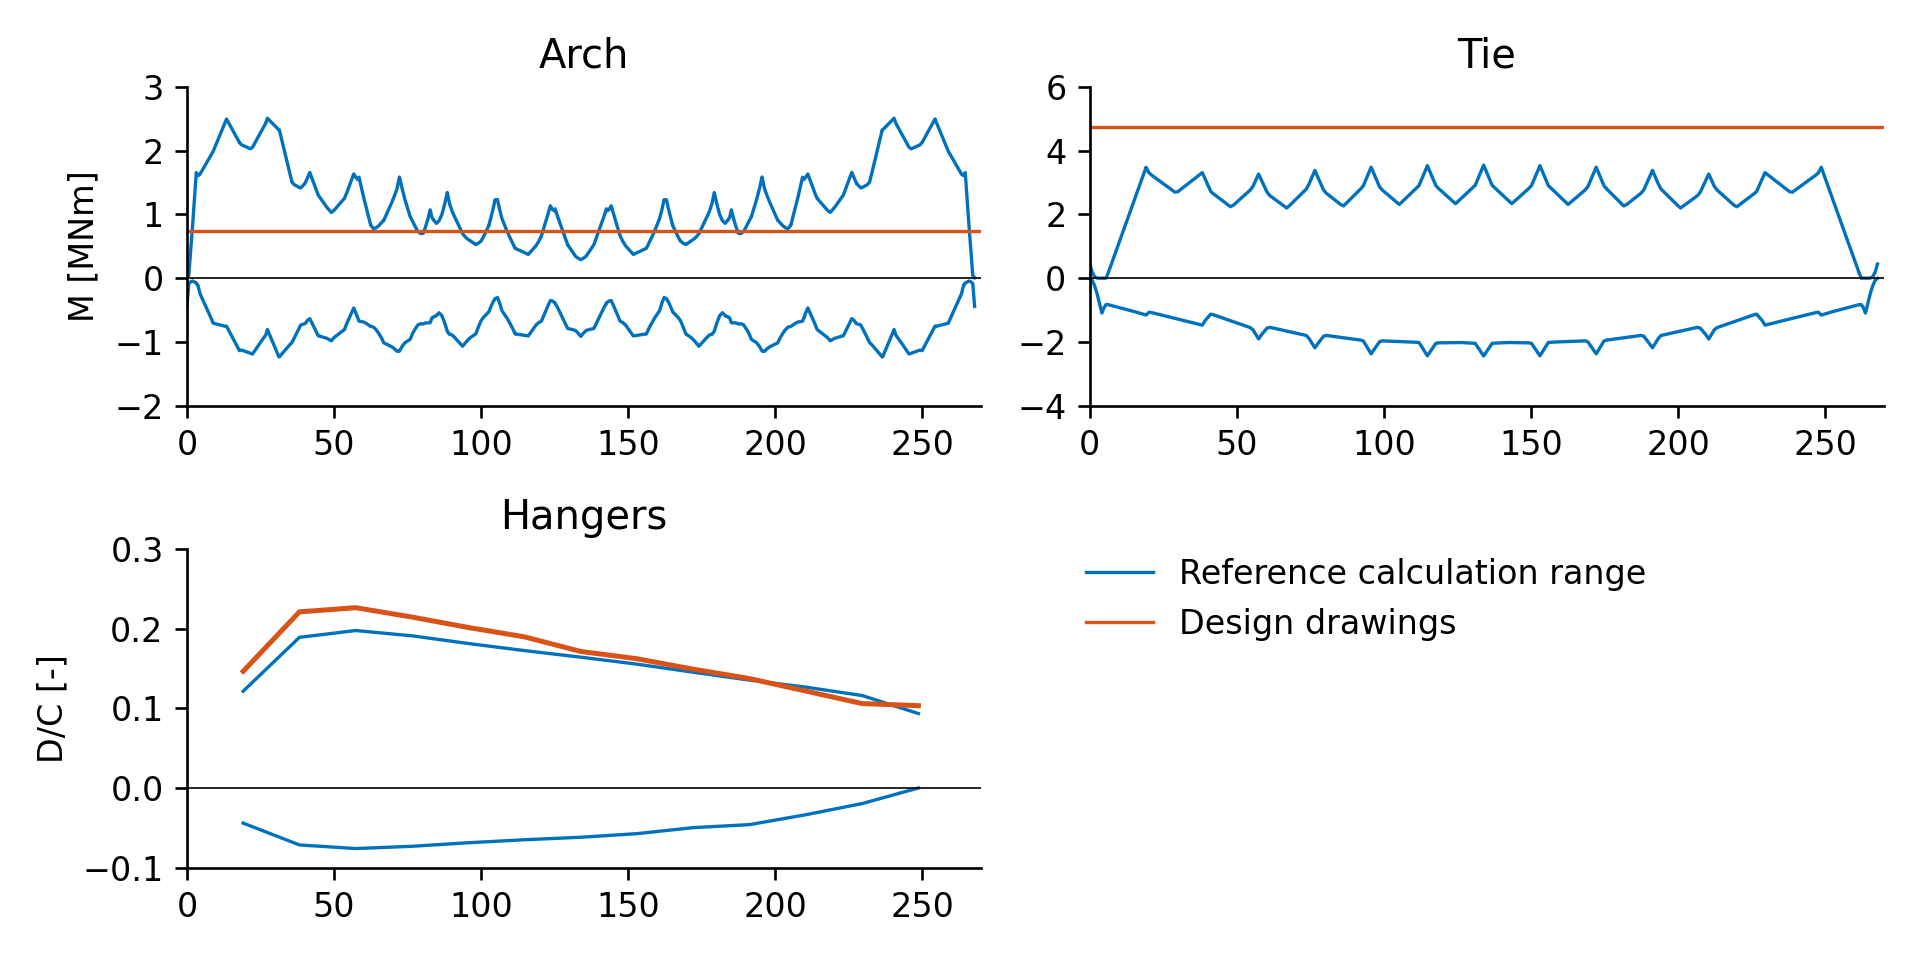
\includegraphics[width=0.8\textwidth]{calculations/Base case/Live load.png}
    \caption{Range of internal forces effects under live loading}
    \label{fig:base_case_live}
\end{figure}

The moments in the arch given in the design drawings do not correspond to the maximum for the considered load case. The considerable difference cannot be explained in another way and seems physically impossible. The moment distribution in the tie and the hangers' normal forces seem to agree on the other hand. Apparently, the live loading is only slightly overestimated in the model, which can be seen particularly well in the hangers' demand over capacity ratios. These differences are accepted, as it is not the goal of this Thesis to reproduce the results from the design drawings. Interestingly, in particular, the arch segment near the knuckle is affected by strong bending moments. On the other hand, in the tie girder, the range of effects under live loading is well distributed. Apparently, the influence lines for the moments in the tie girder at the different cross-girders follow the same shape. For the hangers, it is the second one from the knuckle connected toward the middle of the arch that undergoes the largest normal force. Towards the other side of the hangers set, the hanger forces decrease. The stronger affected hangers have in common that their inclination is closer to the arch's inclination at their respective connection node. The arch is very stiff on axial loading and comparably weaker on perpendicular forces. Therefore, at the arch nodes, smaller displacements in the hanger's direction are expected for the strongly affected hangers, explaining their higher normal forces. Only the first hanger does not follow this rule, which can be explained by its smaller area of influence. \medskip

\newpage
\subsection{Arch shape}
Traditionally, mainly the circle and the parabola have been used as arch shapes. The parabola has served well as a shape for traditional tied-arch bridges with vertical hangers. In this case, the vertical hanger forces on the arch are evenly distributed and the respective thrust line matches the parabola. For network tied-arch bridges, circular shapes have been considered suitable for radial arrangements. In this case, uniform hanger forces cause an approximately radial loading on the arch, which results in a circular thrust line. For a rise to span ratio of 0.2, the two shapes diverge by at most 0.8\% of the span. While this differences might seem negligible on a drawing, the impact of this difference on the arch's moment distribution is significant, as it is bigger than its usual cross-section height. In this section, the arch shape is first investigated individually as it impacts the investigation of all other variables. \medskip

Multiple approaches to determine the arch shape have been introduced in Section \ref{sec:met_arch}. All of them are linked to the thrust line, which is approximately the most efficient shape. The following four arch shapes are compared in this investigation.
\begin{enumerate}
    \item Thrust line: This shape is obtained numerically as the thrust line for the hanger forces obtained from a tie moment optimisation. The respective hanger forces are uniform at $N_p=\SI{2.4}{MN}$ which corresponds to 45\% of their characteristic resistance.
    \item Polynomial thrust line approximation: The above thrust line is approximated by a quartic function. The quartic function is described by Eq. \eqref{eq:polynomial_shape} and the shape parameter $b$. This parameter is obtained by a least squares approximation. It fulfills the conditions $y(0)=r$ and $y(s/2)=0$
    \begin{equation}
        y(x)=r \cdot \left(1 - b \cdot \left(\frac{2\,x}{s}\right)^2 - (1-b) \left(\frac{2\,x}{s}\right)^4 \right)
        \label{eq:polynomial_shape}
    \end{equation}
    \item Spline thrust line approximation: As a second approximation of the thrust line a cubic spline defined by the arch-hanger connection nodes is used. These nodes are therefore represented at their exact location.
    \item Thrust line of continuous hanger arrangement: This shape is the thrust line of the hypothetical continuous hanger arrangement, which was introduced in Section [].
\end{enumerate}

These shapes are hardly distinguishable by eye. To make their differences visible, only their respective deviations to the parabolic shape are shown in Fig. \ref{fig:arch_shapes_13}. Also a circular arch is shown to put the results into perspective.

\begin{figure}[H]
    \centering
    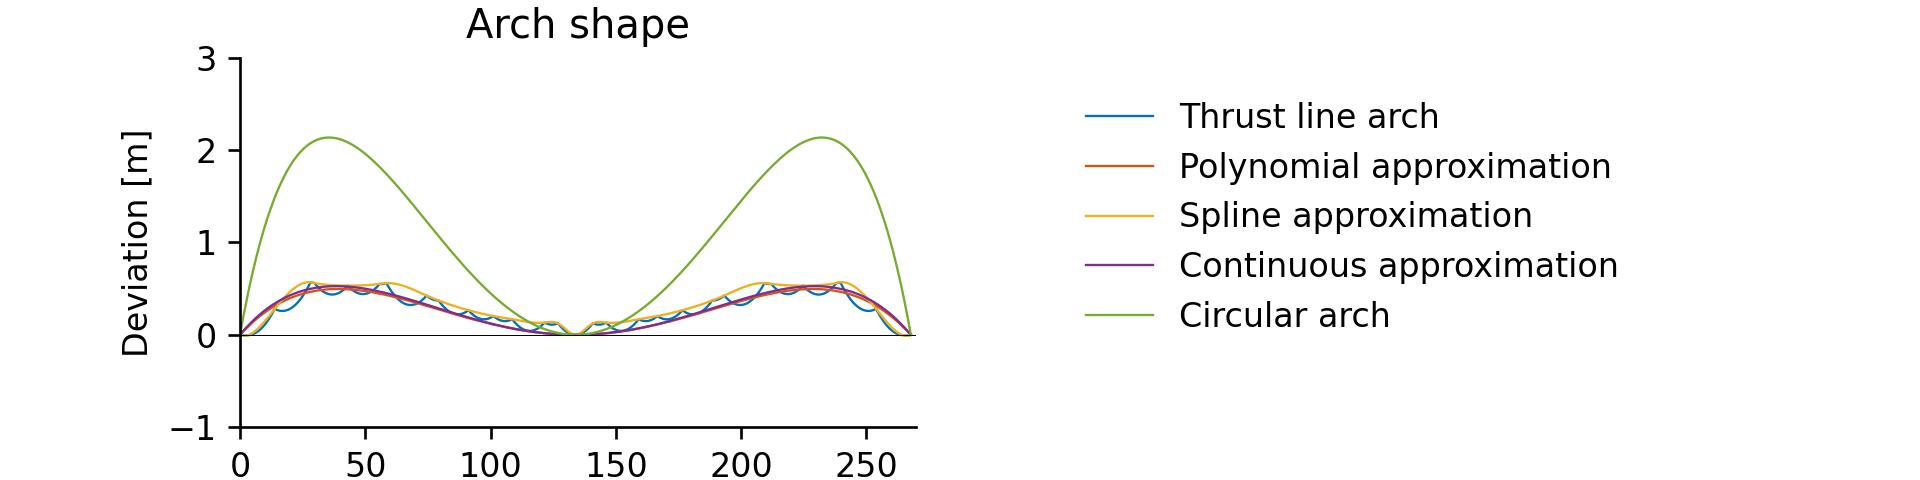
\includegraphics[trim={0 0 2cm 0},clip, width=0.8\textwidth]{calculations/arch shape/arch_shapes_13.png}
    \caption{Deviation of arch shapes from parabolic shape}
    \label{fig:arch_shapes_13}
\end{figure}

In the range between the circular and the parabolic shape, the thrust line tends slightly to the parabolic side. From the similarity between the polynomial and the continuous approximation, it can be concluded, that if the hanger arrangement is dense enough, a quartic function can yield an appropriate arch shape for this hanger arrangement pattern. All three approximations seem to fit the thrust line reasonably well. But to investigate the impacts of the remain deviations from the thrust line, the corresponding permanent moment distribution is presented in Fig. \ref{fig:arch_permanent_moments_13}.

\begin{figure}[H]
    \centering
    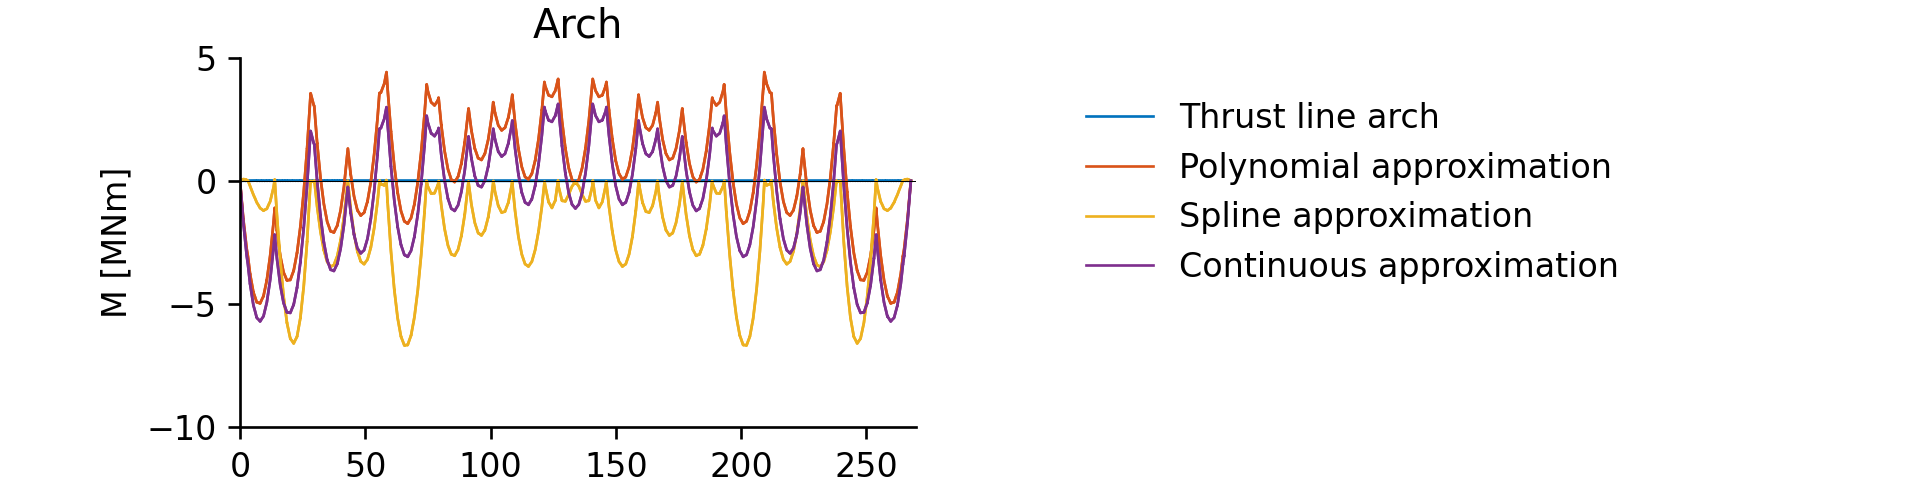
\includegraphics[trim={0 0 2cm 0},clip, width=0.8\textwidth]{calculations/arch shape/permanent state_13.png}
    \caption{Permanent arch moment distributions depending on arch shape}
    \label{fig:arch_permanent_moments_13}
\end{figure}

Despite the apparent match of the arch shapes, significant bending moments result in each of the three approximations. The spline approximation's moment distribution is strictly negative, which relies on the characteristic that a spline lies above the approximately linear thrust line and only matches it at the connection nodes. It is particularly interesting, that all approximations feature a similar parabolic moment distribution between the arch-hanger connection nodes. While these moment distributions resulting for the approximated shapes are certainly considerable, it is practically infeasible to find a simple shape matching the arch thrust line. Any shape with an approximately constant radius $R$ results in a certain deviation from the thrust line and the corresponding moment deviation $\Delta M$. This deviation can be approximated depending on the distance between two hanger points $d$ and the arch's normal force $N$ according to Eq. \eqref{eq:moment_deviation}.

\begin{equation}
    \Delta M=-\left(R-\sqrt{R^2-\left(d/2\right)^2}\right) \cdot N
    \label{eq:moment_deviation}
\end{equation}

For the Blennerhassett Island Bridge, these variables roughly correspond to $R=\SI{194}{m}$, $d=\SI{17}{m}$ and $N=\SI{40}{MN}$. Eq. \eqref{eq:moment_deviation} yields a moment deviation of $\Delta M=\SI{7.5}{MNm}$ coming close to the value observed in Fig. \ref{fig:arch_shapes_13}. From the analytical form of Eq. \eqref{eq:moment_deviation} it can further be concluded, that a reduction of the hanger node spacing has a more than proportional impact on the bending moment deviation. To put these deviations into the context of the design verifications, the demand over capacity ratios resulting in the arch are shown in Table \ref{tab:arch_shape_dc_13} for each approach.

\begin{table}[H]
    \centering
    \input{calculations/arch shape/dc_comparison_13.txt}
    \caption{Arch design verifications considering different shapes}
    \label{tab:arch_shape_dc_13}
\end{table}














\subsection{Hanger density}
It is evident, that an increase of the amount of hangers, can yield a substantial benefit by reducing the decisive effects in the extreme event of cable loss. For the design of the Blennerhassett Island Bridge, a detailed dynamic analysis was conducted, which allowed to reduce the dynamic amplification factor down to 1.6. Nevertheless, the extreme event of cable loss was decisive for the arch segments.

\subsection{Floor beam density}


\newpage
\section{Conclusion}\label{sec:conclusion}

\newpage
\section{Outlook}\label{sec:outlook}

%\newpage
%\input{Section6}                   

%\newpage
%\input{Section7}                   

%\newpage
%\input{Section8}

%\newpage
%\input{Section9}

\clearpage
\appendix
\section*{Appendix}\addcontentsline{toc}{section}{Appendix}
\cleardoublepage
\section{Appendix - Model}
\label{AppendixA}

\subsection{Hanger modelling}
\label{Appendix_A_Hangers}
The initial geometry of the retaining wall is illustrated in Figure

\subsection{Live loading}
\label{Appendx_A_Live_loading}
\begin{table}[H]
\begin{tabular}{cclccccccccc}
\cline{2-11}
             & Lane     &  & 1    & 2    & 3    & 4    & 5    & 6    & 7    & 8    &      \\
             & Reaction &  & 0.91 & 0.80 & 0.69 & 0.57 & 0.46 & 0.35 & 0.24 & 0.13 &      \\ \hline
Loaded Lanes & MPF      &  &      &      &      &      &      &      &      &      & Sum  \\ \hline
1            & 1.2      &  & 10.2 &      &      &      &      &      &      &      & 10.2 \\
2            & 1.0      &  & 8.5  & 7.5  &      &      &      &      &      &      & 16.0 \\
3            & 0.85     &  & 7.2  & 6.3  & 5.5  &      &      &      &      &      & 19.0 \\
4            & 0.75     &  & 6.4  & 5.6  & 4.8  & 4.0  &      &      &      &      & 20.8 \\
5            & 0.70     &  & 6.0  & 5.2  & 4.5  & 3.8  & 3.0  &      &      &      & 22.5 \\
6            & 0.65     &  & 5.5  & 4.9  & 4.2  & 3.5  & 2.8  & 2.1  &      &      & 23.0 \\
7            & 0.60     &  & 5.1  & 4.5  & 3.8  & 3.2  & 2.6  & 2.0  & 1.3  &      & 22.5 \\
8            & 0.55     &  & 4.7  & 4.1  & 3.5  & 3.0  & 2.4  & 1.8  & 1.2  & 0.6  & 21.3 \\ \hline
\end{tabular}
\end{table}

\newpage
\printbibliography
\end{document}
